%%%%%%%%%%%%%%%%%%%%%%% file template.tex %%%%%%%%%%%%%%%%%%%%%%%%%
%
% This is a general template file for the LaTeX package SVJour3
% for Springer journals.          Springer Heidelberg 2010/09/16
%
% Copy it to a new file with a new name and use it as the basis
% for your article. Delete % signs as needed.
%
% This template includes a few options for different layouts and
% content for various journals. Please consult a previous issue of
% your journal as needed.
%
%%%%%%%%%%%%%%%%%%%%%%%%%%%%%%%%%%%%%%%%%%%%%%%%%%%%%%%%%%%%%%%%%%%
%
% First comes an example EPS file -- just ignore it and
% proceed on the \documentclass line
% your LaTeX will extract the file if required
\begin{filecontents*}{example.eps}
%!PS-Adobe-3.0 EPSF-3.0
%%BoundingBox: 19 19 221 221
%%CreationDate: Mon Sep 29 1997
%%Creator: programmed by hand (JK)
%%EndComments
gsave
newpath
  20 20 moveto
  20 220 lineto
  220 220 lineto
  220 20 lineto
closepath
2 setlinewidth
gsave
  .4 setgray fill
grestore
stroke
grestore
\end{filecontents*}
%
\RequirePackage{fix-cm}
%
%\documentclass{svjour3}                     % onecolumn (standard format)
%\documentclass[smallcondensed]{svjour3}     % onecolumn (ditto)
%\documentclass[smallextended]{svjour3}       % onecolumn (second format)
\documentclass[twocolumn]{svjour3}          % twocolumn
%
\smartqed  % flush right qed marks, e.g. at end of proof
%
\usepackage{graphicx}
\usepackage{amssymb}
\setcounter{tocdepth}{3}
\usepackage{listings}
\usepackage{subfigure}
\usepackage{mathtools}
\usepackage{url}
\usepackage{cite}
\urldef{\mailsa}\path|{jbrunelle, mkelly, hany, mweigle, mln}@cs.odu.edu|    
%\newcommand{\keywords}[1]{\par\addvspace\baselineskip\noindent\keywordname\enspace\ignorespaces#1}
\usepackage{colortbl}
\usepackage{color}
\usepackage{alltt}
\usepackage{wrapfig}
\usepackage{amsmath} % Added by MAT 20130711
%\usepackage[noend]{algpseudocode} % Added by MAT 20130711
\usepackage[linewidth=1pt]{mdframed}
\usepackage[numbers]{natbib}

\hyphenation{Web-Cite}
\hyphenation{Java-Script}
\hyphenation{local-host}
\hyphenation{Arch-ive-it}
\hyphenation{Arch-ive-It}
\hyphenation{Ar-chive}
\hyphenation{Time-Map}
\hyphenation{Time-Maps}

\hyphenation{Time-Map}
\hyphenation{Time-Maps}
\hyphenation{Mem-ento}
\hyphenation{Date-time}
\hyphenation{Date-times}
\hyphenation{date-time}
\hyphenation{date-times}
\hyphenation{style-sheet}
\hyphenation{Style-sheet}
\hyphenation{style-sheets}
\hyphenation{Style-sheets}
\hyphenation{Mem-ento-Date-times}
\hyphenation{Mem-ento-Date-time}

%
% \usepackage{mathptmx}      % use Times fonts if available on your TeX system
%
% insert here the call for the packages your document requires
%\usepackage{latexsym}
% etc.
%
% please place your own definitions here and don't use \def but
% \newcommand{}{}
%
% Insert the name of "your journal" with
% \journalname{myjournal}
%
\begin{document}

\title{Not All Mementos Are Created Equal: Measuring The Impact Of Missing Resources}

%\titlerunning{Short form of title}        % if too long for running head

\author{Justin F. Brunelle, Mat Kelly, Hany SalahEldeen, Michele C. Weigle, and Michael L. Nelson}

% the affiliations are given next; do not give your e-mail address
% unless you accept that it will be published
\institute{Old Dominion University, Department of Computer Science\\
Norfolk VA, 23529, USA\\
\mailsa\\}
\date{Received: date / Accepted: date}
% The correct dates will be entered by the editor


\maketitle
\begin{abstract}

Web archives do not always capture every resource on every page that they attempt to archive. This results in archived pages missing a portion of their embedded resources. These embedded resources have varying historic, utility, and importance values. The proportion of missing embedded resources does not provide an accurate measure of their impact on the Web page; some embedded resources are more important to the utility of a page than others. We propose a method to measure the relative value of embedded resources and assign a damage rating to archived pages as a way to evaluate archival success. In this paper, we show that Web users' perceptions of damage are not accurately estimated by the proportion of missing embedded resources. In fact, the proportion of missing embedded resources is a less accurate estimate of resource damage than a random selection. We propose a damage rating algorithm that provides closer alignment to Web user perception, providing an overall improved agreement with users on memento damage by 17\% and an improvement by 51\% if the mementos have a damage delta $\textgreater$0.30. We use our algorithm to measure damage in the Internet Archive, showing that it is getting better at mitigating damage over time (going from 0.16 in 1998 to 0.13 in 2013). However, we show that a greater number of important embedded resources (2.05 per memento on average) are missing over time. Alternatively, the damage in WebCite is increasing over time (going from 0.375 in 2007 to 0.475 in 2014) while the missing embedded resources is remaining constant (~13\% of the resources are missing on average). Finally, we investigate the impact of JavaScript on the damage of the archives, showing that a crawler that can archive JavaScript dependent representations will improve memento damage by 13.5\%.

\keywords{Web Architecture, Web Archiving, Digital Preservation}
\end{abstract}


\section{Introduction}
%\section[This is a very long title i want to break it manually]{This is a very long title\\ i want to break it manually}
\label{introduction}
Web archives are valuable cultural repositories that capture and store Web content. Users make use of archives like the Internet Archive \cite{iawebarchive, waybackarchives2} to retrieve archived material \cite{usingIA, marshalls_social_media_study} for a variety of purposes and in a variety of ways \cite{yasminLinks}. However, the resources being requested by Web users may not be complete; embedded resources are sometimes missing from an archived Web page \cite{ipresArchivability}. Missing embedded resources return a non-200 HTTP status (e.g., 404, 503) when their URI is dereferenced.

Large images are often more important to an archived page's utility than small images. Similarly, stylesheets that format visible content are more important to the representation of the page than stylesheets without significant formatting responsibilities. We provide a mechanism to assess the impact of missing embedded resources in the archives.

Throughout this paper we use Memento Framework terminology. Memento \cite{nelson:memento:tr} is a framework that allows web users to browse in the temporal dimension by aggregating the offerings of the archives at a single point of access. Original (or live web) resources are identified by URI-R, and archived versions of URI-Rs are called \emph{mementos} and are identified by URI-M. Memento TimeMaps are machine-readable lists of mementos (at the level of single-archives or aggregation-of-archives) sorted by archival date.

This research is motivated by three factors. First, we want to understand how missing embedded resources impact Web user satisfaction (i.e., the utility of mementos). Using an algorithm to measure embedded resource importance, we determine whether an important embedded resource of the memento is missing (e.g., a main image or video essential to the user's understanding of the page), or the missing embedded resource is a spacer image or a small button logo that contributes little to the memento's utility for the user. We propose a method of weighting embedded resources in a memento according to importance. We show that this is an improved damage rating over an unweighted count of missing embedded resources. We use Amazon's Mechanical Turk to compare our algorithm to Web users' notion of damage and to show an improvement over the unweighted count of missing embedded resources.

Second, we use our algorithm to assess the damage of mementos in the Internet Archive. We use the unweighted measure of damage as the proportion of missing embedded resources to all requested resources ($M_m$) and compare it to our calculation of damage ($D_m$). %Using this proportion of missing embedded resources as an unweighted comparison baseline, we use our weighting algorithm to determine memento damage in the Internet Archive and use Mechanical Turk to compare the accuracy of each algorithm.

Third and finally, we measure damage in the Internet Archive over time using our weighted algorithm. We then describe how this algorithm can be used for future enhancements of the Heritrix crawler \cite{Sigurosson:Incremental-Heritrix, heritrix} and archival processes.

%In this paper, we examine the results of our work developing an algorithm to accurately measure memento damage (Section \ref{damage}), use Mechanical Turk to evaluate our algorithm against Web user interpretation of damage (Section \ref{turk}), and measure the quality of mementos in the Internet Archive using our algorithm (Section \ref{eval}). 


\section{Motivating Examples}
\label{example}


\begin{figure*}[h!t]
  \begin{center}
    \subfigure[All three of the embedded images are included in $m_0$ and identified by the red arrows (\emph{$M_m$=0.17}).]{\label{undamaged}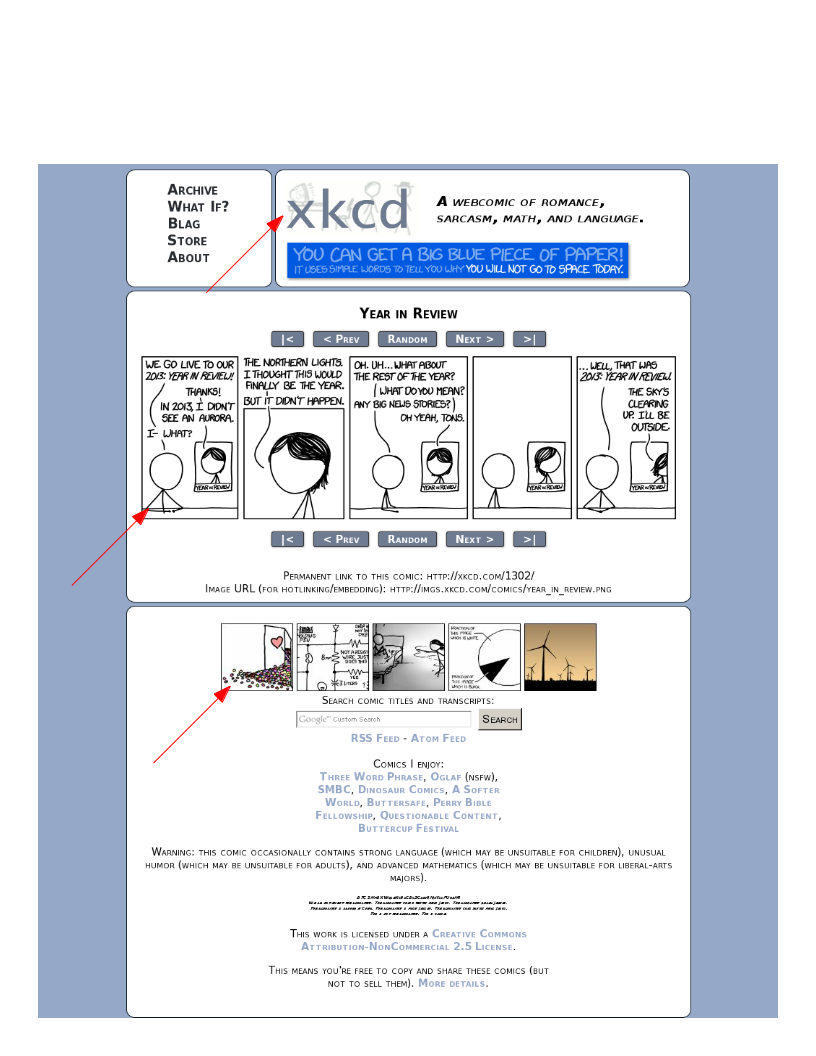
\includegraphics[width=0.3\textwidth]{./imgs/undamagedAnnotated.png}}\qquad
    \subfigure[We removed the large, central image (that is the main content of the page) from $m_1$, identified by the red arrow (\emph{$M_m$=0.24}).]{\label{missingBig}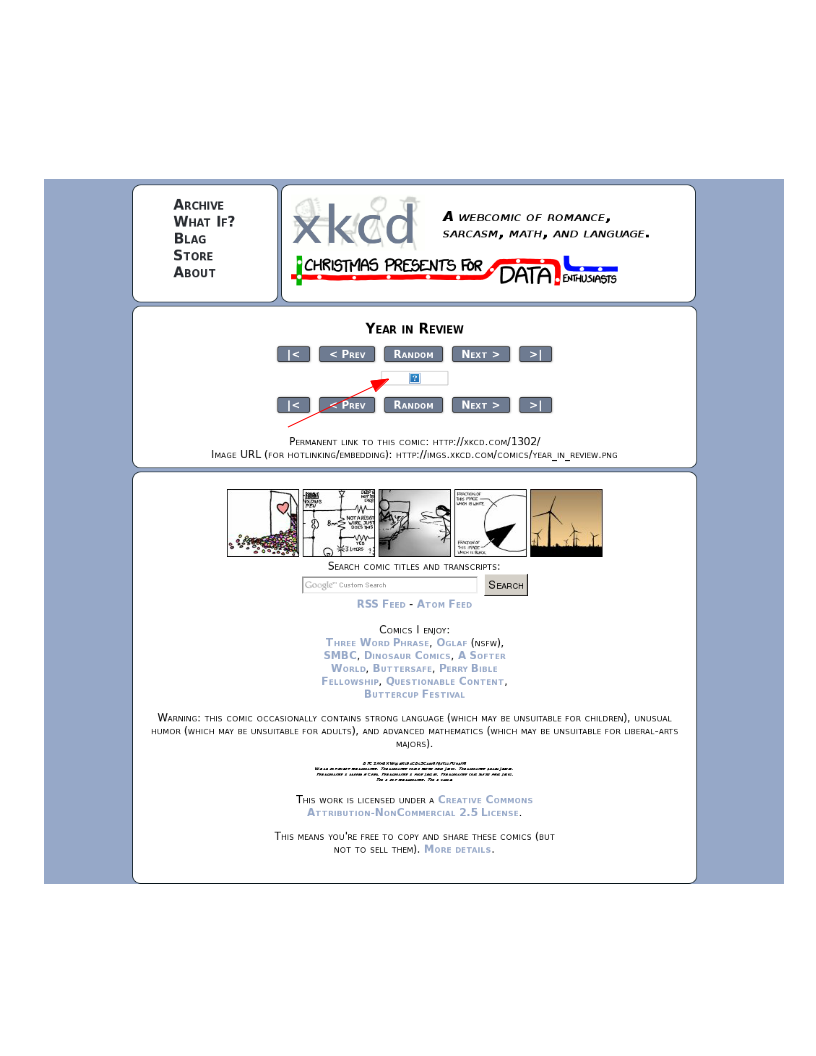
\includegraphics[width=0.3\textwidth]{./imgs/missingBigAnnotated.png}}  \qquad
    \subfigure[We removed the XKCD logo and banner of comics from $m_2$, identified by the red arrows (\emph{$M_m$=0.29}).]{\label{missingLittle}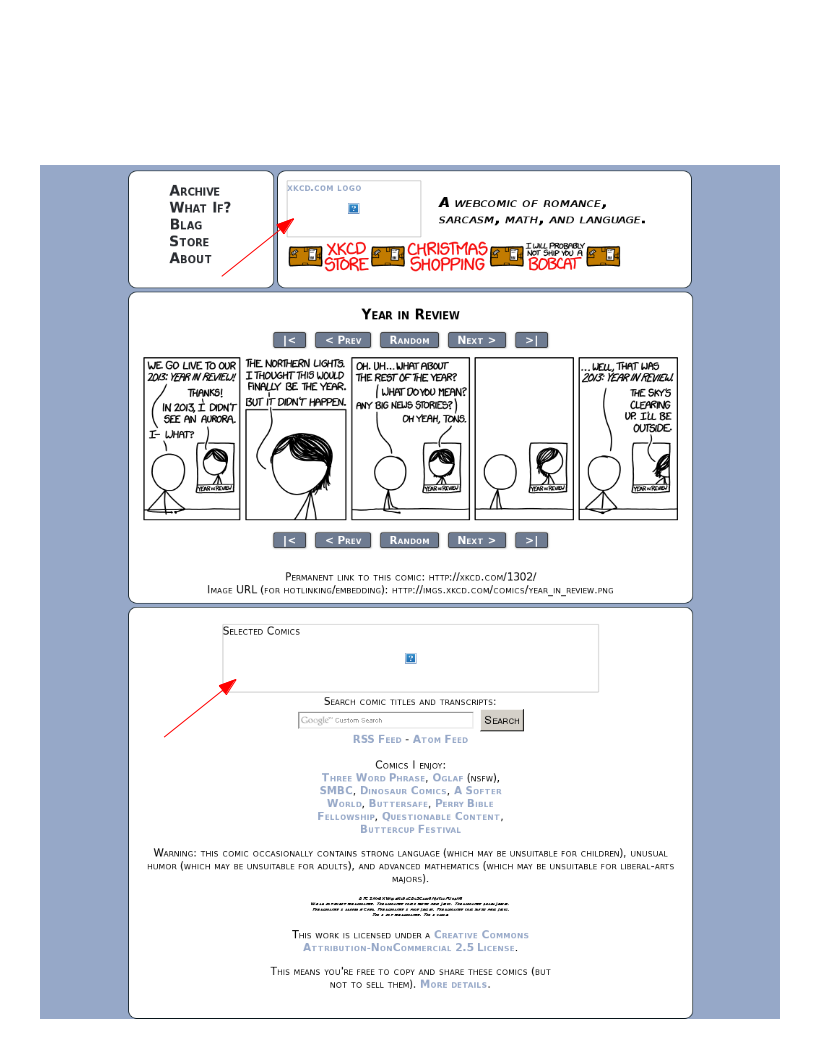
\includegraphics[width=0.3\textwidth]{./imgs/missingLittleAnnotated.png}}  \\
    
    \subfigure[This memento (URI-M \protect\url{http://web.archive.org/web/20110116022653/http://www.cityofmoorhead.com/flood/?}) is missing two stylesheets which changes the entire appearance and utility of the memento (\emph{$M_m$=0.38}).]{\label{missingflood}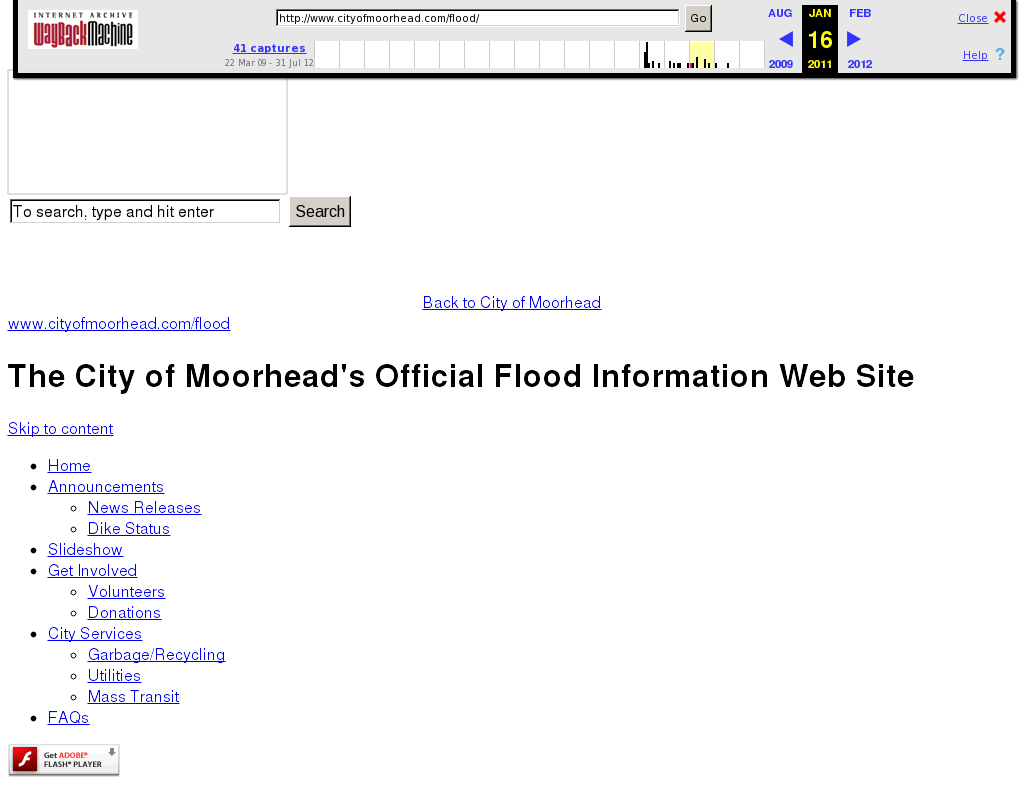
\includegraphics[width=0.45\textwidth]{./imgs/missing_flood_page_crop.png}}\qquad
%,height=8cm,keepaspectratio
    \subfigure[Meanwhile, this memento (URI-M \protect\url{http://web.archive.org/web/20060102083228/http://www.ascc.edu/}) is missing two stylesheets (along with two images) but does not appear damaged (\emph{$M_m$=0.20}).]{\label{missingaldot}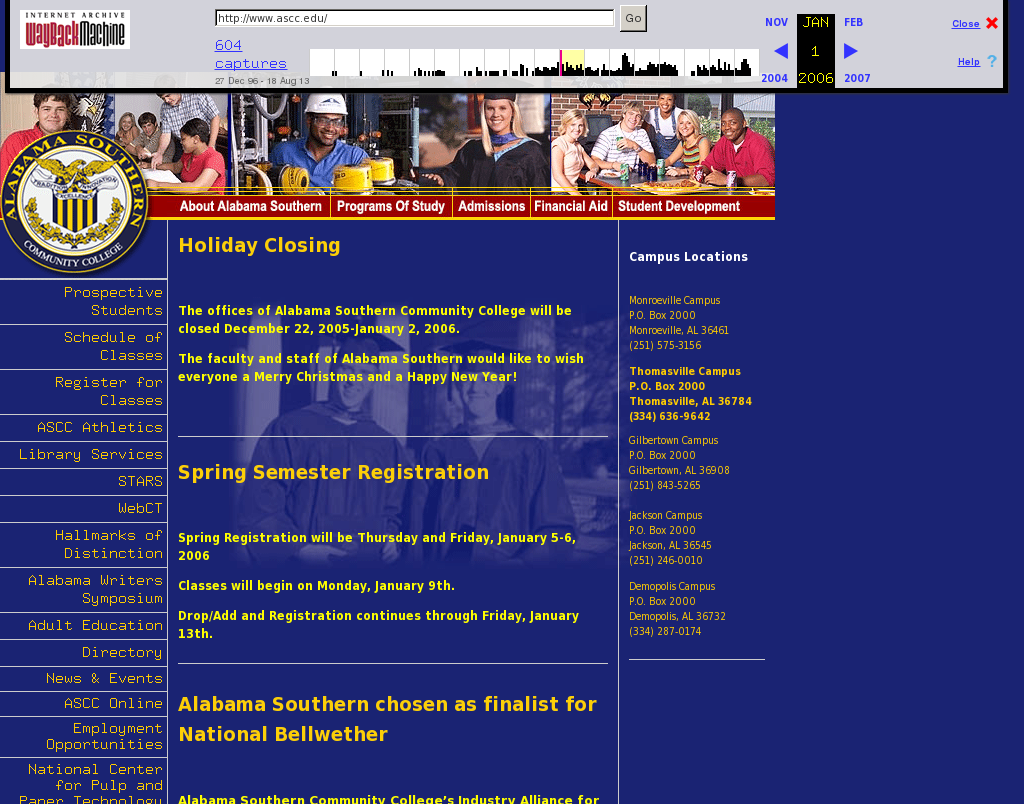
\includegraphics[width=0.45\textwidth]{./imgs/missing_lots_crop.png}}  
  \end{center}
  \caption{Mementos have different meanings and usefulness depending on which embedded resources are missing from the memento (and the proportion of missing resources, $M_m$).}
  \label{xkcdImgs}
\end{figure*}

We use the XKCD Web page as an example of a resource with embedded resources of differing importance. We captured the URI-R using the wget \cite{wget} command\footnote{We executed the wget command with parameters as follows: \texttt{wget -E -H -k -K -p} \url{http://www.xkcd.com/}} and manually inflicted damage on a local memento of \url{http://www.xkcd.com/} by removing embedded images. We used PhantomJS \cite{pjs} to dereference the URI-M, take a PNG snapshot of the representation, and recorded the resulting HTTP response headers of the embedded resources. We created three mementos of the URI-R: one duplicating its live Web counterpart 
%(we call this the \emph{original} memento)
($m_0$), one with the central comic image removed ($m_1$), and one with two logo images removed ($m_2$). The snapshots taken by PhantomJS are provided in Figures \ref{undamaged}, \ref{missingBig}, and \ref{missingLittle}. As shown in the captions, the proportion of embedded missing resources ($M_m$) varies among the mementos.

The live XKCD site is missing two embedded stylesheets, as are $m_0$, $m_1$, and $m_2$ since they are copies of the live resource. We verified that our memento $m_0$ has a $M_m$ value identical to its live Web counterpart -- the live Web resource and $m_0$ are both missing the same embedded resources ($M_m$=0.17). In Figure \ref{undamaged}, $m_0$ has multiple embedded resources, but we focus on the three identified by the red arrows: the XKCD logo, the main comic image, and the banner of comics. The central image is most important to the utility of the page -- without the main comic image, the user does not obtain the information from the page that the author intended (Figure \ref{missingBig}). The logo and banner are not essential to the user's understanding of the XKCD content (Figure \ref{missingLittle}). 

Cascading Stylesheets (CSS) also differ in importance. Some stylesheets are responsible for formatting small portions of a page, while others are responsible for placing images and other content or even organizing the entire page for the user. Figure \ref{missingflood} shows a memento of a URI-R that is missing a single stylesheet. This stylesheet is responsible for a large amount of information in the representation and without it, the meaning and utility of the memento changes. Figure \ref{missingaldot} shows a memento that is properly styled but is missing two stylesheets that are not responsible for the majority of the content organization.% and the memento is still properly styled without them.

As we have discussed, the percentage of successfully dereferenced embedded resources is not the only factor in determining memento quality. In support of that principle, we refer to Figure \ref{missingaldot} in which $M_m$=0.2 (6/30). However, it appears to be well-preserved. In our XKCD example, Figure \ref{missingLittle} is missing two images ($M_m$=0.24) yet maintains more important embedded mementos than Figure \ref{missingBig} ($M_m$=0.29). These examples support the motivation of our research and demonstrate the need for evaluation criteria that assesses perceived memento damage.


\section{Related Work}
\label{priorwork}
Past researchers have studied the completeness of the archives, the recrawl policies that optimize archive quality, and the relative importance of information of content within Web resources. We build upon these prior works and apply their findings to develop our algorithm for automatically assess the quality of mementos.

SalahEldeen et al. have studied the rate at which live resources disappear from the Web. In a study of the Egyptian Revolution, SalahEldeen found that 11\% of the resources shared over Twitter were missing after one year \cite{losingmyrevolution, hanyTPDL2013}. %Studies such as SalahEldeen's show that resources are disappearing from the Web and are inadequately archived. We are investigating how institutions can improve archival quality by assessing the quality of mementos to determine if mementos are adequately archived. 

Our previous work studied the factors influencing archivability, including accessibility standards and their impact on memento completeness \cite{kellyTPDL2013}. In this work, Kelly used a yearly sampling method to select mementos for testing. We use a similar method in this work to study memento damage.

Spaniol has measured the quality of Web archives based on matching crawler strategies with resource change rates \cite{spaniol9catch, spaniol2009data, Denev:2009:SFQ:1687627.1687694}. Ben Saad and Gan\c{c}arski performed a similar study regarding the importance of changes on a page \cite{saad2011}. Gray and Martin created a framework for high quality mementos and assessing their quality by measuring the missing embedded resources \cite{mementoQuality}. While these studies focused on memento completeness and site coverage, we focus on assessing the importance of the artifacts that are missing. 

Fersini et al. studied the importance of information blocks of a rendered Web page, finding that blocks with more images are more important \cite{Fersini20081431}. Singh et al. found that multimedia within a page is essential for user understanding \cite{Singh2009}. Ye et al. found that the information blocks close to the center of the viewport contain important information, while ``noise'' -- or unimportant content -- occurs on the fringes or edges of the page \cite{Yi2003}. Kohlsch\"{u}tter et al. also found that important content was located in the center of pages \cite{boilerPlate}. Centrality is a way for authors to convey importance of information to their users. For example, images in the center of the viewport are more important or contribute to the users' understanding of a page than those positions on the fringes or outside the viewport of a page. Using these prior findings, we constructed an algorithm to assess the importance of embedded resources based on their MIME type, location in the viewport, and size in pixels.

Banos et al. created an algorithm to evaluate archival success based on adherence to standards for the purpose of assigning a resource archivability score \cite{ipresArchivability}. Zhang et al. studied human perception and human ability to recognize differences in images effectively determining human perception limitations for images at the pixel level \cite{Zhang200830}. Rademacher et al. used human perception to identify the visual factors that distinguished computer generated images from photographs \cite{rademacher}. We use human perception in a similar way to identify levels of memento damage.

The algorithm proposed in this paper determines the importance of embedded resources. Song et al. outlined an algorithm for determining the importance of sections of Web pages based on their content, size, and position \cite{blockImportance}. We extend this algorithm (using many of the same principles) to measure the importance of missing embedded resources. 



\section{Users' Perception of Damage}
\label{turk} 

%The damage rating we defined in Section \ref{damage} was constructed from the point of Web archivists; our notions of importance were imbued in the algorithm. Despite supporting evidence (e.g., prior works support our notion that resources centered in the viewport are more important than those on the fringes \cite{Yi2003, boilerPlate}), we needed to validate that our measure of damage matches Web users' interpretation of damage. We used Amazon's Mechanical Turk to evaluate the $D_m$.

As archivists, our perception of damage differs from that of more traditional Web users. To determine if $M_m$ (percent missing) is a good estimate of human perception of damage, we used Amazon's Mechanical Turk to measure human agreement with $M_m$.

To ensure that Mechanical Turk workers (or more colloquially, ``turkers'') could evaluate damage, we presented turkers with pairs of mementos that had varying levels of damage and asked them to select the memento they preferred to keep if given a choice between the two.

We captured 11 manually-selected URI-Rs (Table 1) on a local server and created five versions of the mementos for each URI-R. We manually inflicted damage to the mementos to create the five categories of damage. For the category \emph{missing image}, we removed a prominent image (empirically identified as important) from the memento. For the category \emph{missing css}, we removed a prominent CSS file to cause formatting issues in the memento; we empirically selected the CSS file to remove based on the greatest human-perceived detrimental impact to the page layout. We also created the categories \emph{missing all images} (we removed every embedded image), \emph{missing all resources} (we removed all embedded resources), and \emph{original} (the URI-M was a direct copy of the live resource) and measured the $M_m$ of each URI-M in each category. We refer to the four categories of damaged mementos in aggregate as $m_1$ and the \emph{original} as $m_0$. These categories created a variety of damage ratings by a variety of missing embedded resources for identical URI-Rs at an identical time point to provide a spectrum of damaged mementos for evaluation by turkers.

\begin{table*}[h!t]
\begin{tabular}{ p{6cm} | c |  c |  c |  c |  c }
	 & \multicolumn{5}{c}{$M_m$}\\
    URI-R & $m_0$ & missing image & missing css & missing all images & missing all\\
    	\hline
    	\hline
    \protect\url{http://www.cs.odu.edu/~mln/} & 0.14 & 0.43 & 0.29 & 0.43 & 0.43 \\
    	\hline 
    \url{http://activehistory.ca/2013/06/myspace-is-cool-again-too} \url{-bad-they-destroyed-history-} \url{along-the-way/comment-page-1/} & 0.0 & 0.32  & 0.32 & 0.57 & 0.85 \\
    	\hline
    \protect\url{http://www.albop.com/} & 0.0 & 0.13 & 0.0 & 0.50 & 0.50\\
    	\hline
    \protect\url{http://www.cs.odu.edu/} & 0.10 & 0.13 & 0.11 & 0.82 & 0.81 \\
    	\hline
    \protect\url{http://ws-dl.blogspot.com/2013/08/2013-07-26-web-archiving-and-digital.html} & 0.07 & 0.08 & 0.08 & 0.13 & 0.14 \\
    	\hline
    \protect\url{http://www.cnn.com/2013/08/19/tech/social-media/zuckerberg-facebook-hack/} & 0.19 & 0.22 & 0.28 & 0.46 & 0.57 \\
    	\hline
    \protect\url{http://xkcd.com/} & 0.14 & 0.38 & 0.31 & 0.53 & 0.54 \\
    	\hline
    \protect\url{http://www.mozilla.org/} & 0.80 & 0.80 & 0.80 & 0.877 & 0.89 \\
    	\hline
    \protect\url{http://www.ehow.com/} & 0.05 & 0.05 & 0.06 & 0.11 & 0.33 \\
    	\hline
    \protect\url{http://google.com/}  & 0.0 & 0.0 & 0.0 & 0.0 & 1.0  \\
    	\hline
    \protect\url{http://php.net/} & 0.32 & 0.33 & 0.33 & 0.37 & 0.37  \\
    	\hline
\end{tabular}
  \caption{The 11 URI-Rs used to create the manually damaged dataset. $M_m$ values are provided for each $m_1$.}
  \label{dataset}
\end{table*}

\begin{figure}[h!]
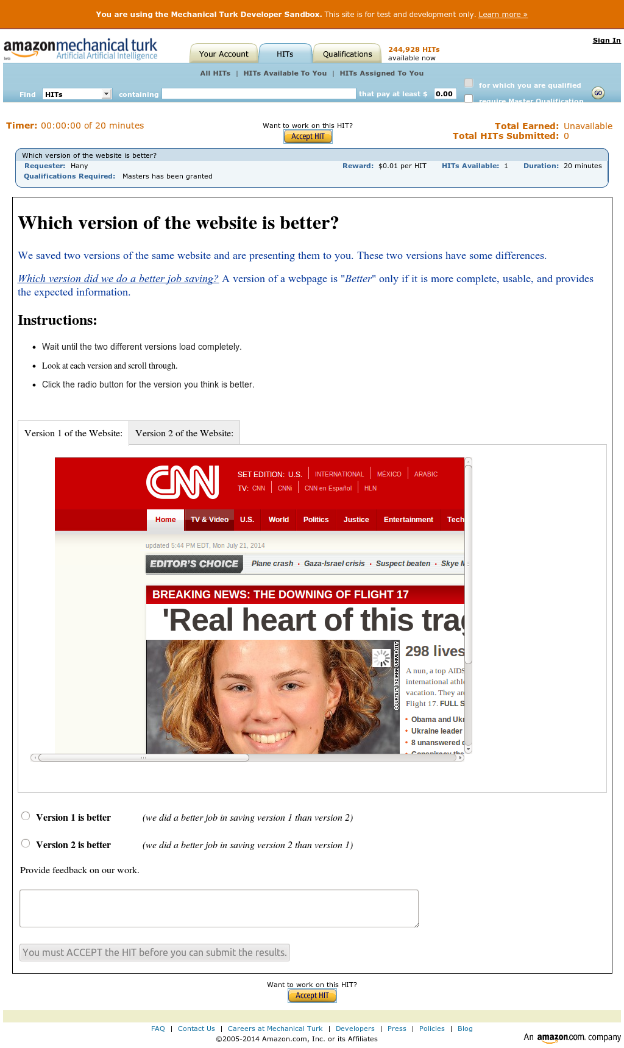
\includegraphics[width=0.50\textwidth]{./imgs/turkss.png}
\caption{We asked the turkers to select the less damaged of two mementos.}
\label{turkss}
\end{figure}


With the goal of determining whether or not turkers can recognize damage in a memento, we presented the turkers with a $m_1$ and its $m_0$ counterpart (that is, a ``damaged'' and its \emph{ground-truth} memento) and asked the turkers ``We saved two pages for you. For which page did we do a better job?'' (Figure \ref{turkss}). For each URI-R, a pair of mementos consisting of $m_0$ and one of the four categories of $m_1$ were evaluated by five turkers for a total of 280 evaluations. 

We show the judgement splits from the turker evaluations in Table \ref{m0table}. The judgement splits refer to the number of turkers that selected the correct-incorrect version. For example, a 0-5 split means all five turkers selected the $m_1$ (an incorrect selection), a 5-0 split means all five turkers selected the $m_0$ memento (the correct selection), and a 3-2 split means three turkers selected the $m_0$ memento and two selected the $m_1$ (a correct selection by the majority, but still a split decision among the turkers). For the purposes of this paper, we consider only 5-0 and 4-1 splits as agreement and all other splits as disagreement. {$\Delta M_m$} refers to the delta between $M_{m_0}$ and $M_{m_1}$.

The turkers selected $m_0$ as the preferred option (less damaged memento) 81\% of the time (226/280). As {$\Delta M_m$} shrinks, turker agreement is more consistent. 


\begin{table}
\begin{tabular}{ c | c | c | c | c | c | c || c}
    {$\Delta M_m$} &  \multicolumn{6}{c}{Splits}\\
  & 5-0 & 4-1 & 3-2 & 2-3 & 1-4 & 0-5 & Total\\
\hline
1.0   &  &  &  &  &  & & 0.00\\
0.9 &  &  &  &  &  & & 0.00\\
0.8 & 4 &  &  &  &  & & 0.07\\
0.7 &  &  &  &  &  & & 0.00\\
0.6 &  &  &  &  &  & & 0.00\\
0.5 & 1 & 1 &  &  &  & & 0.04\\
0.4 &  &  &  &  &  & & 0.00\\
0.3 & 15 & 5 &  &  &  & & 0.36\\
0.2 & 2 &  &  &  &  & & 0.04\\
0.1 & 5 & 4 & 4 & 2 &  & 1& 0.29\\
0.0 & 5 & 3 & 1 & 3 &  & & 0.22\\
\hline
Total & 0.58 & 0.23 & 0.09 & 0.09 & 0.00 & 0.02 & 1.0
\end{tabular}
  \caption{The turkers selected $m_0$ as the preferred memento 81\% of the time, and more consistently for larger {$\Delta M_m$} values.}
  \label{m0table}
\end{table}

%\begin{table}
%\centering
%\begin{tabular}{c >{\bfseries}r @{\hspace{0.7em}}c @{\hspace{0.4em}}c }
%  \multirow{10}{*}{\rotatebox{90}{\parbox{4cm}{\bfseries\centering Turker Assessment}}}
%    & \multicolumn{3}{c}{\bfseries $M_m$}\\
%  & & \bfseries Select $m_0$ & \bfseries Select $m_1$\\
%  & $m_0$ & \MyBox{44}{ } & \MyBox{0}{ }\\[2.4em]
%  & $m_1$ & \MyBox{11}{ } & \MyBox{0}{ }\\
%\end{tabular}
%  \caption{Confusion matrix of the turker assessments of the $m_0$ vs $m_1$ comparison test.}
%  \label{m0cm}
%\end{table}

\begin{table}
\centering\begin{tabular}{cll}
\textbf{Turker} & \multicolumn{2}{c}{ \textbf{ $M_{m}$}}                           \\
\textbf{Assesment}                  &          Select $m_{0}$             &           Select $m_{1}$             \\ \cline{2-3} 
       $m_{0}$           & \multicolumn{1}{|l}{44} & \multicolumn{1}{|l|}{0} \\ \cline{2-3} 
       $m_{1}$           & \multicolumn{1}{|l}{11} & \multicolumn{1}{|l|}{0} \\ \cline{2-3} 
\end{tabular}
 \caption{Confusion matrix of the turker assessments of the $m_0$ vs $m_1$ comparison test.}
  \label{m0cm}
\end{table}


Regardless of {$\Delta M_m$}, 81\% of the evaluations agreed with $M_m$ as a suitable damage metric (5-0 and 4-1 splits). Turkers were unsure about the damage (3-2 and 2-3 splits) 18\% of the time and incorrectly identified damage only once. The average {$\Delta M_m$} for the unsure selections was $\textless$ 0.01, and the only 0-5 split had a {$\Delta M_m$} of 0.014, suggesting that confusion or disagreement occurs more often when the damage delta is smaller. 

Confusion matrices provide a consolidated view of an algorithm's performance. The top left quadrant shows the number of true positives, the top right shows the number of false negatives, the bottom left shows false positives, and the bottom right shows true negatives. The algorithm's accuracy ((True Positives + True Negatives) / (All Positives and Negatives)) and harmonic mean (or $F_1$ Score: 2 * True Positives / (2 * True Positives + False Positives + False Negatives)) are calculated using a confusion  matrix. A harmonic mean provides an average (in this case, of the algorithm's success rate) and is sensitive to small values and outliers.  

From the confusion matrix (Table \ref{m0cm}), we can calculate the accuracy of $m_0$ vs $m_1$ as 0.80 with a harmonic mean of 0.88. Turker agreement does not match $M_m$ 100\% of the time with the $m_0$ vs $m_1$ test because of phenomena with aesthetics and human perception. 

\section{Evaluating Organic Damage}
\label{turkActual}
Turkers identified $m_0$ in the $m_0$ vs $m_1$ in a large majority (81\%) of the comparisons. As a result, the turkers have shown that they can identify a damaged resource when presented a damaged and undamaged memento. Because they can identify damage in mementos, we used turkers to evaluate our measured damage of mementos found in the Internet Archive. 

This experiment uses the same set of 2,000 URI-Rs as in our previous work \cite{ijdl}, which was sampled from Twitter and Archive-It. The first dataset, the \emph{Twitter} set, consists of Bitly URIs shared over Twitter. The second dataset, the \emph{Archive-It} set, was sampled from Archive-It collections. The Archive-It collections are created and curated by human users often corresponding to a certain event (e.g., National September 11 Memorial Museum) or a specific set of Web sites (e.g., City of San Francisco). We discarded non-HTML representations (e.g., JPEG and PDF) from both sets for a final dataset of 1,861 URI-Rs. Non-HTML representations do not contribute to this study since they do not have embedded resources. There is no overlap between the two sets.

Using this set of URI-Rs, we measured the damage of one memento per year from the Internet Archive TimeMap of each of the 1,861 URI-Rs, resulting in 45,341 URI-Ms. We randomly selected a subset of 100 URI-Ms from this set. Similar to the evaluation in Section \ref{turk}, we gave turkers two mementos (we will generalize these to $m_2$ and $m_3$) from consecutive years from the same TimeMap and asked the turkers to select the less damaged memento (``We saved two pages for you. For which page did we do a better job?''). Because $m_2$ and $m_3$ are observed from the Internet Archive, neither is considered a \emph{ground-truth} memento. We measured the damage $M_m$ of mementos in the Internet Archive and compared it to the turker perception of the utility of the mementos. 

Contrary to the test in Section \ref{turk}, as {$\Delta M_m$} grows, the turkers are not as effective at selecting the less damaged memento (the splits are shown in Table \ref{m1table}). The turkers only agree with $M_m$ 12\% of the time and completely disagree with $M_m$ (1-4 and 0-5 splits) 44\% of the time. This discrepancy demonstrates that turker assessment of damage does not match $M_m$. Additionally, we see that the turkers performed well when comparing $m_0$ vs $m_1$ (original vs damaged) but struggle to compare $m_2$ vs $m_3$ (damaged vs damaged).


\begin{table}
\begin{tabular}{ c | c | c | c | c | c | c || c}
    {$\Delta M_m$} &  \multicolumn{6}{c}{Splits}\\
  & 5-0 & 4-1 & 3-2 & 2-3 & 1-4 & 0-5 & Total\\
\hline
1.0 &  &  &  &  & 1 & & 0.01\\
0.9 &  &  &  &  &  & & 0.00\\
0.8 &  &  &  &  &  & & 0.00\\
0.7 &  & 1 &  &  &  & & 0.01\\
0.6 &  &  &  &  & 1 & & 0.01\\
0.5 &  &  &  &  &  & & 0.00\\
0.4 &  & 1 &  &  &  & & 0.01\\
0.3 & 1 &  & 3 & 4 & 1 & 2& 0.11\\
0.2 &  & 5 & 6 & 5 & 12 & 9& 0.37\\
0.1 & 4 & 5 & 10 & 11 & 15 & 3& 0.48\\
0.0 &  &  &  &  &  & & 0.00\\
\hline
Total & 0.05 & 0.12 & 0.19 & 0.20 & 0.30 & 0.14 & 1.0
\end{tabular}
  \caption{The turker evaluations of the $m_2$ vs $m_3$ comparisons when using $M_m$ as a damage measurement.}
  \label{m1table}
\end{table}

\begin{table}
\centering
\begin{tabular}{cll}
\textbf{Turker} & \multicolumn{2}{c}{ \textbf{ $M_{m}$}}                           \\
\textbf{Assesment}                  &          Select $m_{2}$             &           Select $m_{3}$             \\ \cline{2-3} 
       $m_{2}$           & \multicolumn{1}{|l}{29} & \multicolumn{1}{|l|}{24} \\ \cline{2-3} 
       $m_{3}$           & \multicolumn{1}{|l}{23} & \multicolumn{1}{|l|}{24} \\ \cline{2-3} 
\end{tabular}
  \caption{Confusion matrix of the turker assessments of the $m_2$ vs $m_3$ comparison test against $M_m$.}
  \label{m1cm}
\end{table}

%acc = (TP+TN)/(P+N)
%acc = (29+17)/(29+24+23+24)
%f1 = 2tp/(2tp + fp + fn)
%f1 = (2*29)/(2*29 + 23 + 24) 


From the confusion matrix (Table \ref{m1cm}), we can calculate the accuracy of turker selections of $m_2$ vs $m_3$ agreement with $M_m$ is 0.46 with a harmonic mean ($F_1$) of 0.55. In a Receiver Operating Characteristic (ROC) curve \cite{fawcett2006introduction}, we calculated the Area Under the ROC Curve (AUC) for the results of the turker evaluations of $m_2$ vs $m_3$ against $M_m$ and the results of the manually damaged $m_0$ vs $m_1$ test (as the optimal performance). The AUC of $M_m$ is lower (AUC=0.472) than random (AUC=0.500) as shown in Table \ref{auc1}, meaning that $M_m$ performed worse than random for matching turker perception of damage and far worse than the optimal performance (AUC=0.789), a further indicator that $M_m$ is not a suitable metric for measuring memento damage.


\begin{table}
\centering
\begin{tabular}{ c | c | c | c }
    Damage Calculation &  AUC & $F_1$ & Accuracy\\
\hline
  $M_m$ & 0.472 & 0.55 & 0.46\\
  $M_{m_0}$ & 0.789 & 0.88 & 0.80 \\
\hline
\end{tabular}
  \caption{When compared to random, $M_m$ performs worse than random selection and is worse than the optimal performance of $m_0$ vs $m_1$.}
  \label{auc1}
\end{table}



%%%%%%%%%%%%%%%%%%%%%%%%%%%%
%%%%%%%%%%%%%%%%%%%%%%%%%%%%
%%%%%%%%%%%%%%%%%%%%%%%%%%%%

\section{Calculating Memento Damage}
\label{damage}
With $M_m$ not matching Web users' perception of damage, we propose a new algorithm for assessing memento damage. Our proposed algorithm is based on the MIME type, size, and location of the embedded resource.

We define $D_m$ as the damage rating, or cumulative damage, of a memento $m$ in Equation \ref{damageeqn}. $D_m$ is a normalized value ranging from $[0,1]$. We calculate the potential damage of a memento and the actual damage of a memento and express the damage rating as the ratio of actual to potential damage. Notionally, potential damage is the cumulative importance of all embedded resources in the memento, while actual damage is only the importance of those embedded resources that are unsuccessfully dereferenced, or missing.

\begin{equation}
\label{damageeqn}
D_m = \frac{D_{m_{actual}}}{D_{m_{potential}}}
\end{equation}

To determine potential and actual damage, we first define the set of all embedded resources \emph{R} and the set of all missing resources \emph{$R_r$} in Equation \ref{resources}.

\begin{equation}
\label{resources}
\begin{split}
R &= \{\text{All embedded resources requested}\}\\
R_r &= \{\text{All missing embedded resources}\}\\
&R_r \subseteq R
\end{split}
\end{equation}

We calculate the importance of each embedded resource in the set \emph{R}. The sum of each embedded resource is the potential damage \emph{$D_{m_{potential}}$} (Equation \ref{potentialdamage}). Important resources are assigned additional weights to increase their relative value over unimportant resources (Equations \ref{imagedamage} - \ref{cssdamage}).

\begin{equation}
\label{potentialdamage}
\begin{split}
D_{m_{potential}}& = \frac{\sum_{i=1}^{n_{[I,MM]}} D_{[I|MM]}(i)}{n_{[I|MM]}} +\frac{\sum_{i=1}^{n_C} D_C(i)}{n_C} %\frac{\sum_{i=1}^{n_{MM}} D_{MM}(i)}{n_{MM}}\\& + D_T(M)\\&\forall\{\text{I=Images, MM=Multimedia, C=CSS}\}\\& n \in R
\\&\forall\{\text{I=Images, MM=Multimedia, C=CSS}\}\\& n \in R
\end{split}
\end{equation}

Actual damage ($D_{m_{actual}}$, defined in Equation \ref{actualdamage}) is identical to $D_{m_{potential}}$ except it is computed using only the missing embedded resource set \emph{$R_r$}. %As shown in Equation \ref{damageeqn}, the damage rating is the ratio of actual damage to potential damage.

\begin{equation}
\label{actualdamage}
\begin{split}
D_{m_{actual}} =& \frac{\sum_{i=1}^{n_{[I,MM]}} D_{[I,MM]}(i)}{n_{[I|MM]}} + \frac{\sum_{i=1}^{n_C} D_C(i)}{n_C} %\frac{\sum_{i=1}^{n_{MM}} D_{MM}(i)}{n_{MM}}\\& + D_T(M)\\&\forall\{\text{I=Images, C=CSS, MM=MultiMedia}\} \\&n \in R_r
\\&\forall\{\text{I=Images, MM=Multimedia, C=CSS}\} \\&n \in R_r
\end{split}
\end{equation}


In $M_m$, all embedded resources are treated as equal; all embedded resources are assigned a value of 1 with $weight$=1.0 applied. The potential damage is therefore the number of embedded resources, and the actual damage is the number of missing embedded resources. $M_m$ is the unweighted ratio of missing embedded resources to total embedded resources.

We assign additional weights to important embedded resources at the expense of less important mementos. When a weight $w$ is given to an embedded resource, all $n$ embedded resources lose $\frac{w}{n}$ importance, which redistributes the importance between embedded resources while keeping the sum of all importance constant. Images receive weights for image size and centrality (Equation \ref{imagedamage}). We use the pixel area (width $x$ height) of the image and the page size along with a weight for horizontal and vertical central dividing line overlap by the image.

\begin{equation}
\label{imagedamage}
\begin{split}
&D_{[I|MM]} = 1 + \frac{width * height}{\text{Page Size (pixels)}}\\ &+ (w_{\text{horizontal}} \iff \text{Overlaps horizontal center})\\
&+ (w_{\text{vertical}} \iff \text{Overlaps vertical center})\\
&w_{\text{horizontal}} = 0.25\\
&w_{\text{vertical}} = 0.25
\end{split}
\end{equation}

%&+ ({w_{centrality}}{2} \iff \text{Overlaps vertical middle})\\

Embedded multimedia importance ($D_{MM}$) is calculated identically to image importance $D_I$, and we represent both in the same equation $D_{[I|MM]}$. Because size and centrality determine multimedia importance, we omit audio and other non-visual multimedia resources. We also classify Flash movies as multimedia.

%\begin{equation}
%\label{mmdamage}
%\begin{split}
%D_{MM} &= 1 + \frac{width * height}{\text{Page Size}}\\ &+ (\frac{w_{centrality}}{2} \iff \text{Overlaps horizontal middle})\\
%&+ (\frac{w_{centrality}}{2} \iff \text{Overlaps vertical middle})\\
%w_{centrality} &= 0.50
%\end{split}
%\end{equation}


Equation \ref{cssdamage} outlines the damage from missing stylesheets, including a factor for a style threshold $w_{style}$. 


\begin{equation}
\label{cssdamage}
\begin{split}
D_C &= 1 + w_{style} \iff\\&(\text{\textgreater 75\% non-background in
 left two columns}) 
\\& + w_{tags} \iff\\&(\text{tags in the DOM
 without matching CSS})\\
w_{style} &= 0.50\\
w_{tags} &= 0.50
\end{split}
\end{equation}


Our intuition is that a missing important stylesheet will shift content to the left of the page rather than center content in the viewport, we divide a PNG snapshot of a memento into vertical thirds and measure the amount of content in each third. Traditional Web design (and particularly design enabled by stylesheets) evenly distributes content across each of the vertical thirds. If a stylesheet is missing \emph{and} content appears to be shifted to primarily the left two-thirds, we assume the missing stylesheet was important to the distribution of content on the page.

When detecting content in the PNG snapshot, we use remaining CSS files and the HTML to determine the background color of the page. We measure the number of background and non-background colored pixels, with content being the number of non-background colored pixels. The proportion of non-background colored pixels in each vertical third gives us the amount of content in each partition.

The style threshold is determined as follows:

\begin{enumerate}
  \item Determine background color
  \item Render a PNG snapshot of the page
  \item Divide PNG into vertical third partitions
  \item Calculate number of pixels of the non-background color in each third for the viewport only (we used a 1024x768 viewport) and entire page
  \item If $\le$75\% of the non-background colored pixels are in the left two thirds of the viewport, set \emph{$w_{style}=0$} in Equation \ref{cssdamage} (CSS file does not receive a weight)
  \item If $>$75\% of the non-background colored pixels are in the left two thirds of the viewport and left two thirds of the entire page and a stylesheet is missing, \emph{$w_{style}=0.5$} in Equation \ref{cssdamage} (CSS file does receive a weight)
\end{enumerate}

For example, we created two mementos of the URI-R \url{http://www.pilotonline.com/} on a local server, one as it appears live (with all stylesheets -- Figure \ref{withcss2}) and the other with its stylesheets removed (Figure \ref{withoutcss2}). The vertical partitions extend from the top of the PNG snapshot to the bottom.
 The percent of non-background color pixels in the viewports of our mementos are shown in their respective thirds in Figure 2. Notice that the non-background pixels (text, images, etc.) shift left when the CSS is missing. Intuitively, information is not meant to be displayed like the content in Figure \ref{withoutcss2}.

\begin{figure}[h!]
  \begin{center}
    \subfigure[We calculated that the non-background color is more evenly distributed between the three vertical partitions of the Pilot Online page with its stylesheet included than when it is missing.]{\label{withcss2}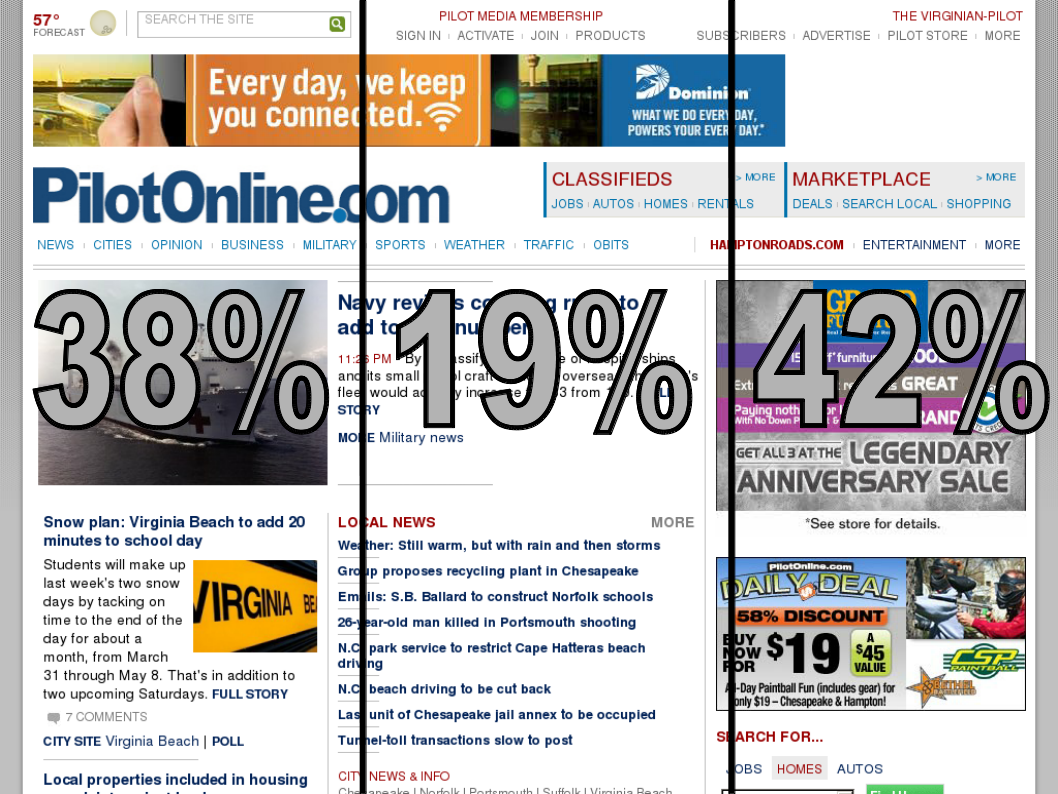
\includegraphics[width=220px]{./imgs/withcss.png}}\\
    \subfigure[We calculated that the non-background color is most prevalent in the left-most vertical partition of the viewport of the Pilot Online page when it is missing its stylesheet.]{\label{withoutcss2}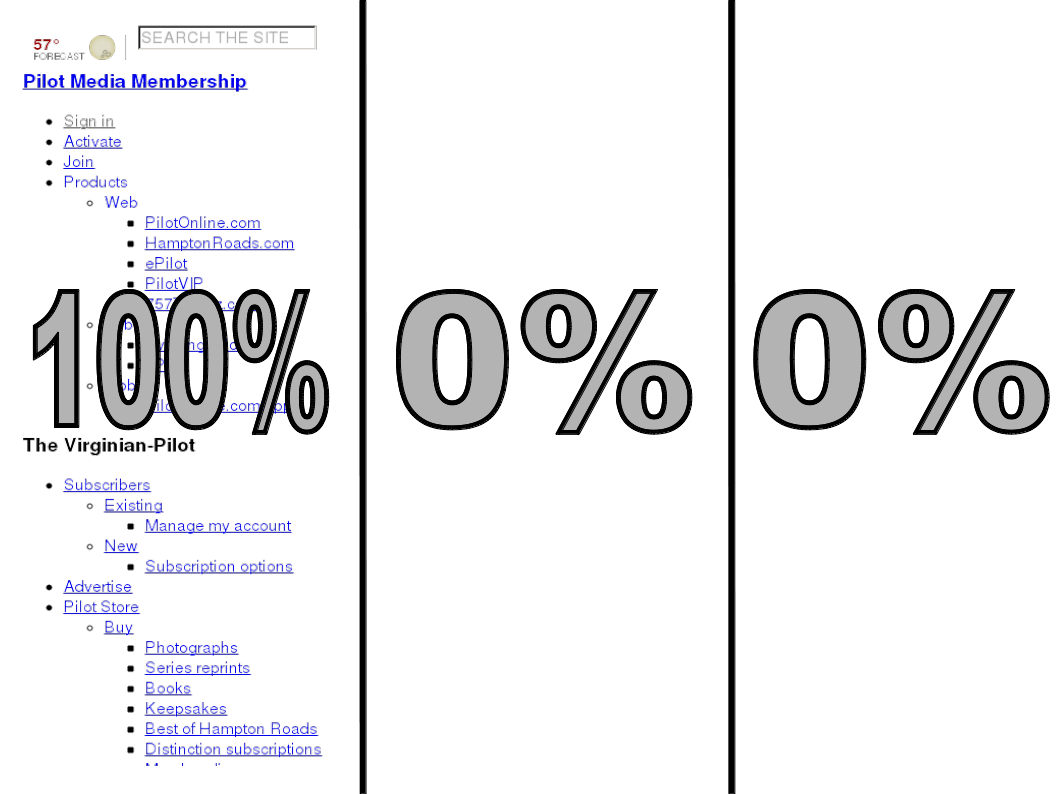
\includegraphics[width=220px]{./imgs/nocss.png}}  
  \end{center}
  \label{pilotexample2}
  \caption{Missing stylesheets causes content to shift left. We show the percent of content in the vertical partitions of the viewport.}
\end{figure}

When we consider content outside of the viewport (Figures \ref{withcss} and \ref{withoutcss}), we see the same shift of content to the left when stylesheets are missing. However, the distribution of content in Figure \ref{withoutcss} is more evenly distributed because the content has shifted down and fills out the middle and right vertical partitions more than in Figure \ref{withoutcss2}. This is an indicator that the stylesheets missing in Figures \ref{withoutcss2} and \ref{withoutcss} were important.

\begin{figure}[h!]
  \begin{center}
    \subfigure[When considering the entire page, the content of the page is distributed 33\% in the left, 26\% in the middle, and 41\% in the right partitions when the stylesheet is present.]{\label{withcss}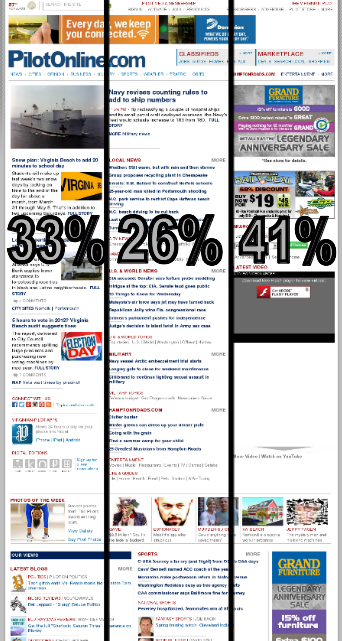
\includegraphics[width=100px]{./imgs/thePng_crop3.png}}\qquad
    %{\label{withcss}
\includegraphics[width=0.2\textwidth]{./imgs/thePng_crop2.png}}\qquad
    \subfigure[When considering the entire page, the content of the page is distributed 84\% in the left, 15\% in the middle, and 1\% in the right partitions when the stylesheet is missing.]{\label{withoutcss}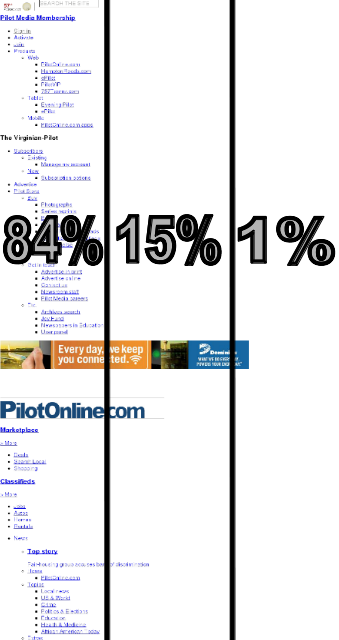
\includegraphics[width=100px]{./imgs/thePngNOCSS_crop3.png}}  
    %{\label{withoutcss}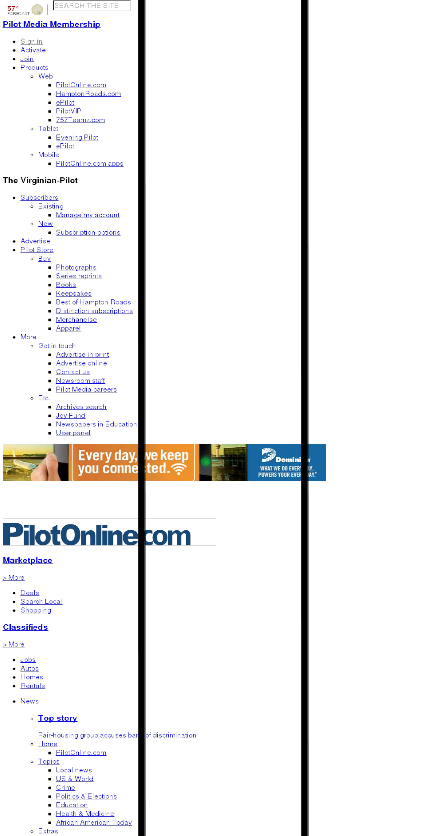
\includegraphics[width=0.2\textwidth]{./imgs/thePngNOCSS_crop2.png}}  
  \end{center}
  \label{full}
  \caption{Missing stylesheets causes content to shift left.We show the percent of content in the vertical partitions of the page.}
\end{figure}


Along with the style threshold, the presence of tags on the page without a matching style suggests that the missing CSS contained the referenced formatting. If such tags exist without a matching style, $w_{tags}=0.5$ in the Equation \ref{cssdamage}. 

Embedded multimedia, images, and stylesheets do not account for the entirety of a page's importance and usefulness. We assume that text, as defined by the DOM and included on the page, is available regardless of archival success and therefore does not contribute to the damage calculation.

%Text plays an important role in a page's informational importance. We determine the importance text plays on a page in relation to the amount of images on a page. We determine the number of words on the page ($NW$), and use the adage \emph{a picture is worth 1,000 words} as the word-to-image ratio $WPI$, giving us the importance of the text $D_T$.

%\begin{equation}
%\label{textdamage}
%\begin{split}
%NW &= \text{Number of Words from Tag-Stripped HTML}\\
%WPI &= \text{1,000 Words/Image (images text is ``worth'')}\\
%D_T &= \frac{NW}{WPI}
%\end{split}
%\end{equation}

%To normalize the damage rating of the page due to the weighting assigned, we take the sum of all potential damages (with weighting assigned) of all embedded resources. We then determine the base value of each memento based on this increased value and normalize the values of the embedded resources. 
%For example, if a page has two embedded resources, \emph{a} and \emph{b}, and \emph{a} is assigned a 0.5 additional importance weight, the total calculated importance will be 2.5 (\emph{a=1.5}, \emph{b=1}). The normalized value for each embedded resource will be 2/2.5=0.8. This makes \emph{a}=1.2 and \emph{b}=0.8 for a total potential damage of 2 which normalizes to 1 for the page.

Equations \ref{damageeqn} - \ref{cssdamage} are used to compute $D_m$:

\begin{enumerate}
  \item Load URI-M with PhantomJS
  \item Find Potential Damage $D_{m_{potential}}$ (\ref{damageeqn})
  \begin{enumerate}
	\item Determine CSS importance $D_C$ (\ref{cssdamage})
	\item Determine Multimedia importance $D_{MM}$ (\ref{imagedamage})
	\item Determine Image importance $D_I$ (\ref{imagedamage})
  \end{enumerate}
  \item Determine proportion of unsuccessfully dereferenced embedded resources $M_m$
  \item Find Actual Damage $D_{m_{actual}}$ (same as Step 3, but with only those URI-Ms unsuccessfully dereferenced)
  \item Determine total damage $D_m$=[0,1] (\ref{damageeqn})
  \
  %\item Print report
  %\begin{enumerate}
	%\item  URI-Ms and associated damage $D_{[C, MM, I]}$=[0,1]
	%\item  Total Page Damage $D_{URI-M}$=[0,1]
	%\item  Percent resources missing $M$=[0,1]
  %\end{enumerate}
\end{enumerate}


With $D_m$ defined, we revisit the examples presented in Section \ref{example}. The values for $D_m$ and $M_m$ are listed in Table \ref{damageTable}. Note that the damage ratings are closer to our empirical human assessment of memento quality than the proportion of the missing embedded resources.

\begin{table}
\centering
\begin{tabular}{ c | c | c }
    \hline
    Figure & $D_m$ & $M_m$\\
    \hline
    \hline
\ref{undamaged} & \emph{0.09} & \emph{0.17}\\
\ref{missingBig} & \emph{0.41} & \emph{0.24}\\
\ref{missingLittle} & \emph{0.36} & \emph{0.29}\\
\ref{missingflood} & \emph{0.59} & \emph{0.38}\\
\ref{missingaldot} & \emph{0.003} & \emph{0.20}\\
    \hline
\end{tabular}
  \caption{$D_m$ vs $M_m$ for the images in Figure \ref{xkcdImgs}. Note $M_m \textgreater D_m$ in 2 of 5 cases.}
  \label{damageTable}
\end{table}

Not all pages and page construction methods can be evaluated by this algorithm. An edge case not handled by this algorithm is any page constructed with iframes. Our algorithm uses JavaScript to determine the rendered location of embedded multimedia and images. When the embedded media is in a page embedded within another page, our algorithm does not provide the accurate rendered location. For this reason, we exclude iframes from our algorithm. We also exclude missing audio-only multimedia since the sound has no visual impact on the page, and sensory importance beyond sight is not considered in this algorithm.

While $D_m$ includes multimedia calculations, multimedia resources are rarely embedded in our mementos (only observed twice in our entire set of 45,341 URI-Ms). We observed that multimedia is often loaded by JavaScript files embedded in the document object model (DOM); this prevents the multimedia files from being loaded into the archives since archival crawlers (at the time of this experiment) do not execute client-side JavaScript and therefore do not discover the requested files.% (similar to the URI-M \url{http://web.archive.org/web/20131211191109js_/http://pilotonline.com/sites/all/themes/hamptonroads/js/jquery.youtube.player.js}).
\\
\\
\section{Damage in the Archives}
\label{eval} 

Having defined an algorithm for measuring $D_m$, we measured $D_m$ values for each of the 45,341 URI-Ms from Section \ref{turkActual}. We used these measurements to assess $D_m$'s performance relative to turker assessment and perform damage measurements in the Internet Archive.

\subsection{Turker Assessment of $D_m$}
\label{turkerDm}


We compared $D_m$ to turker assessment and $M_m$. As shown in Table \ref{m2table}, $D_m$ agrees with turker assessment of damage 32\% of the time, an increase of 18\% over $M_m$. Additionally, 49\% tie with a 3-2 or 2-3 split and only 16\% of the turker evaluations disagreed with the $D_m$ measure. Turkers agree more consistently when {$\Delta D_m$} is larger. If we only consider {$\Delta D_m \textgreater$} 0.30, the turkers agree with $D_m$ 71\% of the time. However with {$\Delta M_m \textgreater$} 0.30, the turkers agree only 20\% of the time. 


\begin{table}
\begin{tabular}{ c | c | c | c | c | c | c || c}
    {$\Delta D_m$} &  \multicolumn{6}{c}{Splits}\\
  & 5-0 & 4-1 & 3-2 & 2-3 & 1-4 & 0-5 & Total\\
\hline
1.0 &  &  &  &  &  & & 0.00\\
0.9 &  & 1 &  &  &  & & 0.01\\
0.8 &  &  &  &  &  & & 0.00\\
0.7 &  &  &  &  &  & & 0.00\\
0.6 &  &  & 1 &  &  & & 0.01\\
0.5 &  &  &  &  &  & & 0.00\\
0.4 & 4 & 1 &  &  &  & & 0.05\\
0.3 & 2 & 2 & 3 &  &  & & 0.07\\
0.2 &  & 2 & 1 & 2 & 2 & 1& 0.08\\
0.1 & 4 & 16 & 27 & 15 & 12 & 3& 0.77\\
0.0 &  &  &  &  &  & & 0.00\\
\hline
Total & 0.10 & 0.22 & 0.32 & 0.17 & 0.14 & 0.04 & 1.0
\end{tabular}
  \caption{The turker evaluations of the $m_2$ vs $m_3$ comparisons when using $D_m$ as a damage measurement.}
  \label{m2table}
\end{table}



\begin{table}
\centering
\begin{tabular}{cll}
\textbf{Turker} & \multicolumn{2}{c}{ \textbf{ $D_{m}$}}                           \\
\textbf{Assesment}                  &          Select $m_{2}$             &           Select $m_{3}$             \\ \cline{2-3} 
       $m_{2}$           & \multicolumn{1}{|l}{45} & \multicolumn{1}{|l|}{32} \\ \cline{2-3} 
       $m_{3}$           & \multicolumn{1}{|l}{8} & \multicolumn{1}{|l|}{14} \\ \cline{2-3} 
\end{tabular}
  \caption{Confusion matrix of the turker assessments of the $m_2$ vs $m_3$ comparison test against $D_m$.}
  \label{m2cm}
\end{table}



%acc = (TP+TN)/(P+N)
%acc = (45+14)/(45+8+14+32)
%f1 = 2tp/(2tp + fp + fn)
%f1 = (2*45)/(2*45 + 8 + 32) 

%we see the accuracy of $m_2$ vs $m_3$ against $M_m$ is 0.46 with a harmonic mean of 0.55

From the confusion matrix in Table \ref{m2cm}, we determine that the accuracy of $D_m$ when comparing $m_2$ vs $m_3$ is 0.60, and the harmonic mean is 0.69. This is an improvement of 0.14 over the accuracy of $M_m$ and an improvement over the harmonic mean of $M_m$ by 0.14, showing that $D_m$ measures damage closer to turker perception. 
We also calculated the AUC in a ROC curve for $D_m$ and compared it to $M_m$ and the optimal performance of the $m_0$ vs $m_1$ test. As shown in Table \ref{auc2}, $D_m$ has an AUC of 0.584, an increase in 0.108 over $M_m$, showing that $D_m$ outperforms $M_m$ and is closer to the optimal performance of $m_0$ vs $m_1$ (AUC=0.789).


\begin{table}
\centering
\begin{tabular}{ c | c | c | c }
    Damage Calculation &  AUC & $F_1$ & Accuracy\\
\hline
  $M_m$ & 0.472 & 0.55 & 0.46 \\
  $D_m$ & 0.584 & 0.69 & 0.60 \\
  $M_{m_0}$ & 0.789 & 0.88  & 0.80 \\
\hline
\end{tabular}
  \caption{$D_m$ provides a closer estimate of turker perception of damage and our optimal performance of $m_0$ vs $m_1$ than $M_m$.}
  \label{auc2}
\end{table}

\subsection{Measuring the Internet Archive}
\label{missing}

With $D_m$ validated as aligning closer to turker evaluations than $M_m$, we used $D_m$ to evaluate the Internet Archive's performance. Our measurement shows that only 46\% of the 45,341 URI-Ms listed in the 1,861 TimeMaps are complete -- that is, 54\% of all URI-Ms listed in the Internet Archive TimeMaps we studied are missing at least one embedded resource\footnote{The Internet Archive performs URI canonicalization very well, and is assumed to not be a source of missing resources.}. In Figure \ref{missingByYear}, we show the average number of missing embedded resources $M_m$ along with the average calculated damage $D_m$ per URI-M per year.

%We also include vertical lines that identify major Heritrix software releases that correspond to changes in changes to the trajectory of memento damage averages across the archive.

\begin{figure}[h!]
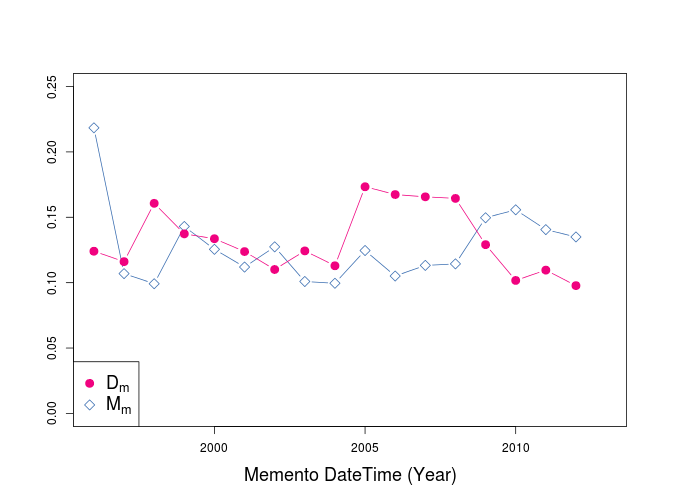
\includegraphics[width=270px]{./imgs/missedAndDamagePerYear.png}
%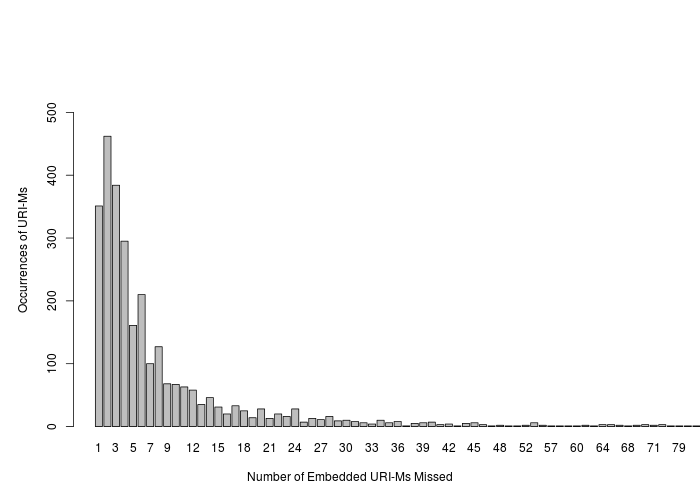
\includegraphics[width=0.50\textwidth]{./imgs/occStats.png}
\caption{The average embedded resources missed per memento per year as compared to damage per memento per year ($\overline{D_m}$=0.128, $\overline{M_m}$=0.132).}
\label{missingByYear}
\end{figure}


Because the number of missed mementos is important to $M_m$ and $D_m$, we investigated the occurrence of missing and successfully dereferenced embedded resources. Most mementos are missing very few embedded resources with most missing 1-10 embedded resources (Figure \ref{missingDistro}), ($\mu=1.7$, $\sigma=4.6$). We calculate that 61\% of mementos are missing 3 or fewer embedded resources, and 85\% of mementos are missing 6 or fewer embedded resources. While the number of successfully dereferenced embedded resources in mementos is more evenly distributed (Figure \ref{foundDistro}), most mementos have very few embedded resources ($\mu=17.6$, $\sigma=86$).

\begin{figure}[h!]
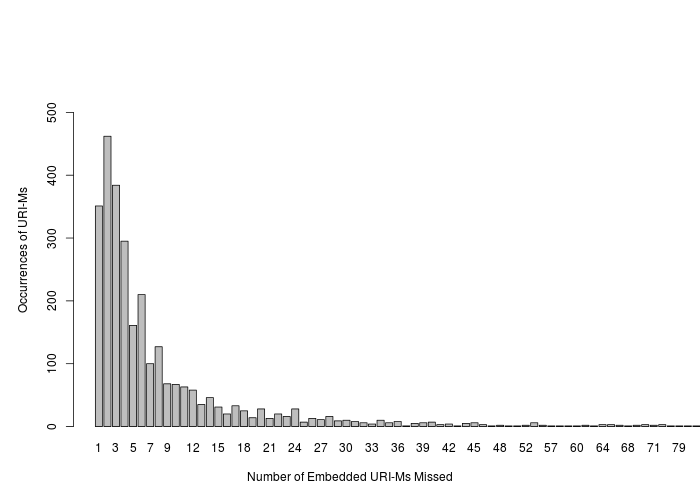
\includegraphics[width=270px]{./imgs/occStats.png}
\caption{The distribution of the number of missing embedded resources per URI-M.}
\label{missingDistro}
\end{figure}

\begin{figure}[h!]
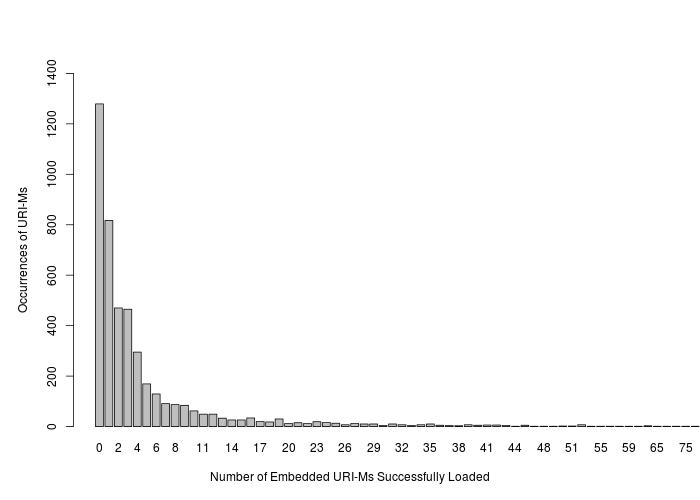
\includegraphics[width=270px]{./imgs/occStatsFound.png}
\caption{The number of successfully dereferenced resources is more evenly distributed than those missing (Figure \ref{missingDistro}).}
\label{foundDistro}
\end{figure}

%\subsection{Measured Damage}
%\label{archiveDamage}


In aggregate, we observed that 45,009 of 292,192 embedded resources were missing, meaning 15\% of the embedded resources in the dataset are missing. Of these, 25,848  (57\% of the missing URI-Ms) were important, meaning they were assigned an additional weight by $D_m$ (Equations 5 and 6). The average damage of all measured mementos was 0.132.

The yearly $\overline{D_m}$ goes from an average of 0.16 in 1998 to 0.13 in 2013. That means the Internet Archive is doing a better job (over time) reducing the total memento damage in its collection. However, the number of missing \emph{important} resources (resources with an importance $\textgreater 1$ due to added weights) is increasing, going from an average of 1.30 important resources per memento in 1997 to 2.38 important resources per memento in 2013 for an average of 2.05 missing per memento. Meanwhile, the number of unimportant missing embedded resources (damage rating $\leq 1$) per memento is increasing at a lesser rate, going from 1.35 in 1997 to 1.64 in 2013. This suggests that while the Internet Archive is getting better overall at mitigating damage as much as possible, the archive is missing an increasing number of embedded resources deemed important. 

The distribution of file types missing per memento (Figure \ref{occstats}) shows that most URI-Ms are missing $\ge 1$ embedded resource and that stylesheets and JavaScript files are increasingly missing over time. Missing JavaScript may lead to additional missing files (such as multimedia). Images are missing at varying rates per memento.

\begin{figure}[h!]
%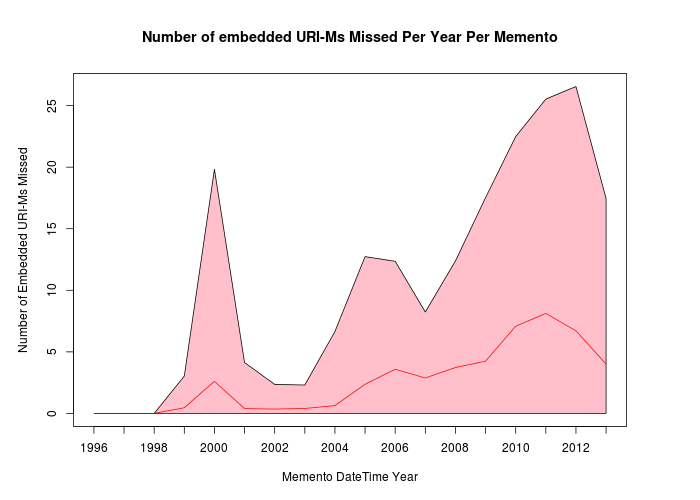
\includegraphics[width=0.5\textwidth]{./imgs/numMissedYearlyPerMem.png}
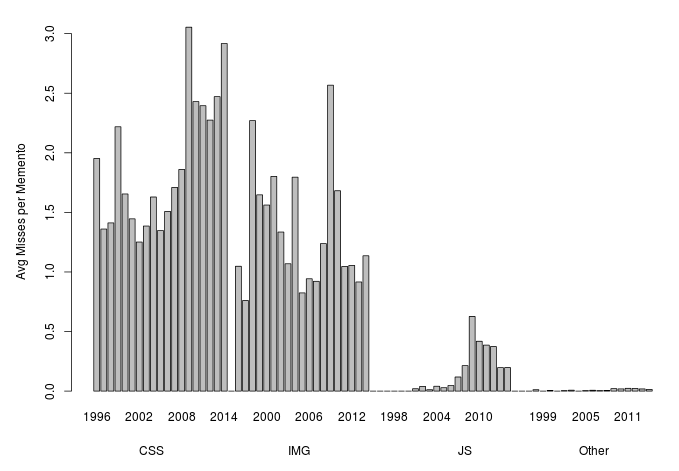
\includegraphics[width=270px]{./imgs/fileTypes.png}
\caption{The number of missed embedded resources per memento per year and MIME type.
%The average is given as the red line, and the standard deviation is the pink area around the average line.
}
\label{occstats}
\end{figure}



\subsection{Measuring WebCite}
\label{webcite}

In an effort to measure a less prominent and different type of archive, we used the damage algorithm to determine $M_m$ and $D_m$ of WebCite\footnote{\url{http://webcitation.org/}}\cite{webcite}. WebCite is different from the Internet Archive's Heritrix crawler in that it is a page-at-a-time archiving tool that creates mementos upon user request. While the Internet Archive's goal is to archive the Web using the Heritrix crawler to identify crawl targets, add their URI-Rs to a crawl frontier, and crawl the frontier, WebCite and other page-at-a-time archivers allow users to submit URI-Rs for archiving, and WebCite immediately archives the resource\footnote{The Internet Archive has recently added an \emph{on-demand} archiving utility at \url{http://archive.org/web/} under the heading ``Save Page Now.''}. When using a page-at-a-time archival service, the resulting memento contains embedded resources with the same archival datetime \cite{temporalCoherence}. This section identifies our damage measurement of this page-at-a-time archiver and outlines the differences between Heritrix and WebCite. 

Our WebCite dataset has 992 mementos in the TimeMaps of our collection of 1,861 URI-Rs. The earliest available memento is from 2007, and the latest is from 2014. Only six mementos are available from 2014; therefore, we will focus on 2007-2013 as the target years of investigation due to the limited number of 2014 mementos, as well as to match the period of observation of the Internet Archive. The average $D_m$ of the collection over all years is $\mu=0.397$ ($\sigma=0.194$), and the average  $M_m$ is $\mu=0.176$ ($\sigma=0.0926$). All of the mementos in this collection are missing at least one embedded resource -- 100\% of the mementos are incomplete. 

As shown in Figure \ref{missingByYearWC}, the average $D_m$ in WebCite is increasing over time, going from 0.285 in 2007 to 0.442 in 2013. Meanwhile, the average $M_m$ remains steady, going from 0.135 in 2007 to 0.139 in 2013. Only slight variation occurs, peaking at 0.287 in 2011. 

Compared to the Internet Archive, WebCite has a higher damage value as well as is missing a larger percentage of embedded resources. Additionally, the damage rating per memento is higher, indicating that a larger percentage of missing embedded resources are important (3,514 or 41.7\%) in WebCite than in the Internet Archive.

\begin{figure}[h!]
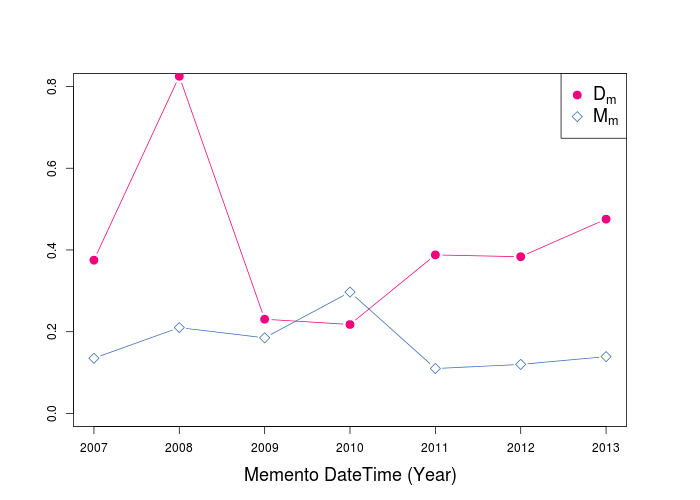
\includegraphics[width=270px]{./imgs/MissedAndDamagePerYear_webcite.png}
%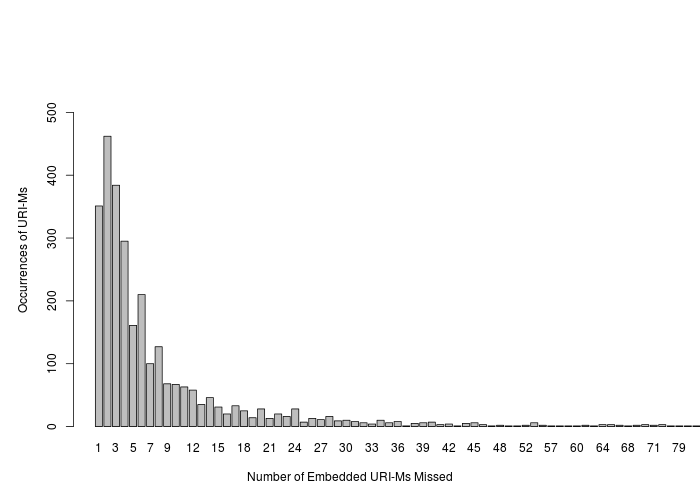
\includegraphics[width=0.50\textwidth]{./imgs/occStats.png}
\caption{The average embedded resources missed per memento per year as compared to damage per memento per year ($\overline{D_m}$=0.397, $\overline{M_m}$=0.176).}
\label{missingByYearWC}
\end{figure}

WebCite is missing on average 10.1 embedded resources per memento ($\sigma=8.0$). Across the entire collection, 8,420 of 54,824, or 15.4\% of the embedded resources were missing in our investigation. We calculate that 56\% of mementos are missing 3 or fewer embedded resources, and 74\% of mementos are missing 6 or fewer embedded resources (Figures \ref{missingDistroWC} and \ref{foundDistroWC}).

\begin{figure}[h!]
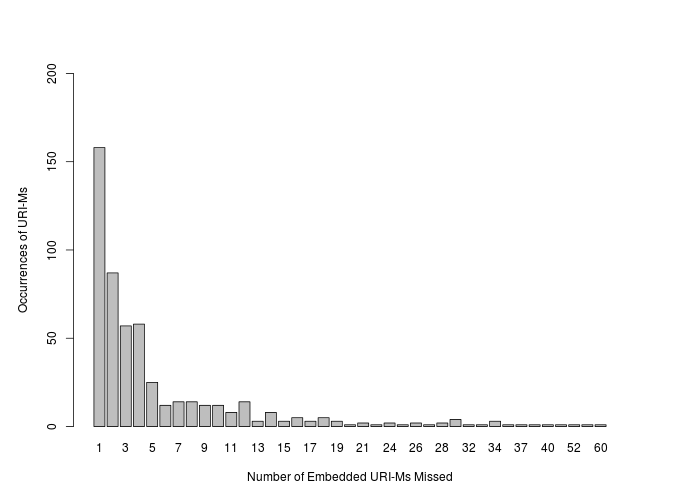
\includegraphics[width=270px]{./imgs/OccStats_webcite.png}
\caption{The distribution of the number of missing embedded resources per URI-M in WebCite.}
\label{missingDistroWC}
\end{figure}


\begin{figure}[h!]
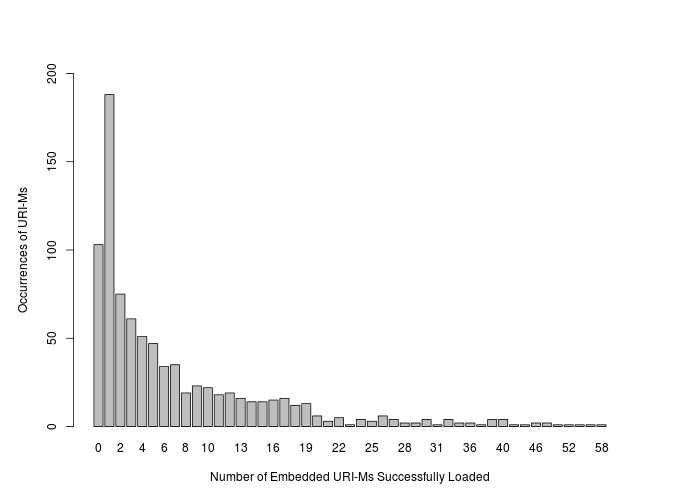
\includegraphics[width=270px]{./imgs/OccStatsFound_webcite.png}
\caption{In WebCite, the number of successfully dereferenced resources is more evenly distributed than those missing (Figure \ref{missingDistroWC}).}
\label{foundDistroWC}
\end{figure}

%\subsection{Measured Damage}
%\label{archiveDamage}


The distribution of file types missing per memento (Figure \ref{occstatsWC}) shows that most URI-Ms are missing $\ge 1$ embedded image and CSS resources, on average. WebCite has a lower occurence of missing stylesheets, but a higher occurrence of missing images. This will impact future work with $D_m$. If we change the weighting of the importance of missing embedded resources -- if we weight missing CSS as having a higher impact on overall $D_m$, WebCite's collection might have a lower average $D_m$. However, more investigation is needed before this conclusion may be reached. 

Our previous investigation \cite{ijdl} showed that WebCite has difficulties when encountering JavaScript and embedded iframes. However, its archiving policies provide immediate results as opposed to crawlers that may incur delay between the time a URI-R is added to the frontier and a memento is created. WebCite's difficulties with JavaScript may contribute to the missing embedded resources if they were loaded through JavaScript.


\begin{figure}[h!]
%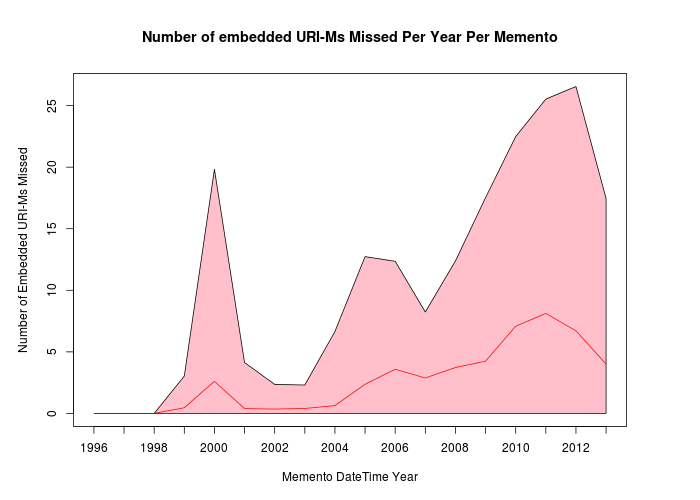
\includegraphics[width=0.5\textwidth]{./imgs/numMissedYearlyPerMem.png}
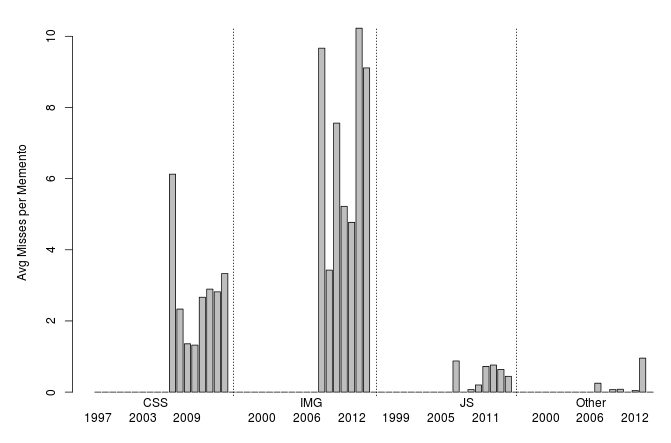
\includegraphics[width=270px]{./imgs/FileTypes_webcite.png}
\caption{The number of missed embedded resources per WebCite memento per year and MIME type.
%The average is given as the red line, and the standard deviation is the pink area around the average line.
}
\label{occstatsWC}
\end{figure}


\section{Impact of JavaScript on Damage}
\label{wcjs}


As a preliminary investigation of the impact of JavaScript on archival tools, we set up an experiment to use Heritrix and PhantomJS \cite{pjs} to crawl the same set of URI-Rs and measure the damage difference between the two set of mementos. Our goal is to understand how $D_m$ is impacted by JavaScript by comparing mementos archived by a crawler that can execute JavaScript (PhantomJS) and a crawler that does not execute JavaScript (Heritrix).

\subsection{PhantomJS vs Heritrix}
\label{pjsvhtrix}
Web crawlers operate by starting with a finite set of seed URI-Rs in a frontier -- or list of crawl targets -- and add to the frontier by extracting embedded URIs in the representations of the URI-R. This allows archival crawlers to discover embedded resources as well as new URI-Rs to crawl while creating mementos. 

Representations of Web resources are increasingly reliant on JavaScript and other client-side technologies to construct a representation. Web browsers use a JavaScript engine to execute the client side code, but Web crawlers traditionally do not have such an engine or the ability to execute client-side code. As a result, crawlers are unable to discover the resources requested via Ajax and, therefore, are not adding these representations to their crawl frontiers. The crawlers are missing the JavaScript-dependent embedded resources which ultimately causes the mementos of the crawled resources to be incomplete and have higher $D_m$.

To mitigate the impact web developers' practice of using JavaScript and Ajax to load embedded resources, crawlers like Heritrix \cite{htrixJS} have constructed approaches for extracting links from embedded JavaScript to be added to crawl frontiers. Google has also make an investment in indexing deferred representations by using headless browsers like PhantomJS \cite{googleJS}.

Because archival crawlers' abilities differ from the abilities of browsers, the archives currently hold a representation of the Web from the point of view of crawlers and not Web users. In other words, what we archive is increasingly different than what users experience. The intuitive solution to this challenge of archiving deferred representations is to provide crawlers with a JavaScript engine and allow headless browsing (i.e., allow a crawler to operate as would a browser) using a technology such as PhantomJS.

\subsection{Crawling Deferred Representations}
\label{crawlDeferred}
We sampled 50 URI-Rs by randomly generating Bitly.com URIs and identifying the URI-Rs to which the bitly URIs redirected. We then classified the 50 URI-Rs as having deferred representations and crawled the set of URIs with Heritrix and PhantomJS. 

During the Heritrix crawl, we used the 50 URI-Rs as a set of seed URIs and allowed Heritrix to create their mementos. The final frontier size of this crawl was 1,588 URIs of embedded resources used to create the mementos. Using our damage algorithm, we measured the damage of the mementos created by Heritrix and found that $\overline{D_m}$=0.148. Recall that the measured avarage damage of the Internet Archive was 0.13.

To ensure the crawler executes JavaScript and captures JavaScript-dependent resources during the creation of mementos, we then crawled the 50 URI-Rs with PhantomJS. We recorded the embedded resources needed to create the representation, including those originating from JavaScript. This created a frontier of 3,364 URIs which we used as a seed URI list in Heritrix. We then used Heritrix to create the mementos using only the seed URI list, effectively creating mementos using the frontier list of PhantomJS. The damage of the mementos from this crawl was, on average, 0.1291. 

PhantomJS provided a 13.5\% improvement to the collection damage over Heritrix. This provides further evidence that JavaScript-dependent representations reduce the quality of mementos due to traditional crawlers' inability to execute JavaScript.

Not only does using PhantomJS provide a larger crawl frontier, but the damage rating of the resulting mementos is lower. In short, this initial investigation suggests that using PhantomJS mitigates the impact of JavaScript on resources with deferred representations and results in higher-quality mementos.

\section{Measuring Archive.today}
\label{archivetoday}
Archive.today \cite{archivetoday} is another page-at-a-time archival service like WebCite. While WebCite does not properly archive deferred representations, Archive.today creates mementos that limit leakage and missing embedded resources typically occurring in other archival services that ignore JavaScript. To study the impact of Archive.today's handling of JavaScript on memento quality, we submitted each of our 1,861 URI-Rs to the Archive.today service (much like the way Mink performs user-initiated archiving \cite{mink}) to create mementos of each resource. 

When Archive.today creates a memento, it modifies the DOM to remove references to embedded resources that were not available at archive time (i.e., embedded resources that returned a non-200 HTTP response code) \cite{refreshZombies}. This results in a memento that -- if created properly -- has no missing embedded resources. Additionally, Archive.today obfuscates the URIs of embedded mementos, preventing a reliable mapping from URI-R to URI-M. Due to these two archival practices, the damage algorithm used in this paper is ineffective for determining memento quality. For this reason, we alter the method of measuring the effectiveness of Archive.today's archival process. 

We initiated the archiving of each URI-R in our collection by Archive.today. We counted the number of embedded resources that were successfully loaded into the live resources (i.e., returned an HTTP 200 response when their URIs were dereferenced) and compared this number to the number of embedded resources successfully archived by Archive.today. It is worth noting that the delta between the number of embedded resources in live resources and mementos is a measure of neither $M_m$ nor $D_m$, but is instead a mechanism for understanding memento fidelity. 

We found that Archive.today has a delta of $\mu=19.9$ ($\sigma=39.2$), meaning on average, Archive.today did not archive 19.9 embedded resources from the live page due to either its inability to archive the resources, or because Archive.today may have deemed the embedded resources not suitable for archiving\footnote{Archive.today lists the resources it saves and does not save in its FAQ page at \url{http://archive.today/faq.html}}. A histogram of all deltas is provided in Figure \ref{athisto}.

\begin{figure}[h!]
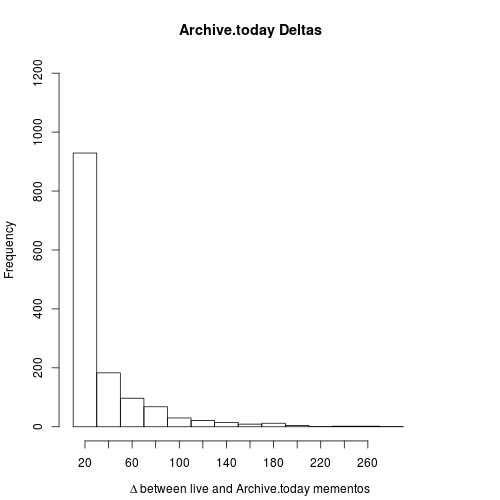
\includegraphics[width=270px]{./imgs/atHisto.png}
\caption{Histogram of the memento vs live resource deltas in Archive.today.}
\label{athisto}
\end{figure}

We submitted each URI-R in the collection to WebCite and recorded deltas for the WebCite mementos in the exact way we measured deltas for Archive.today. In this way, we can compare the two page-at-a-time archiver to determine which service creates higher fidelity mementos. WebCite has a delta of $\mu=21.6$ ($\sigma=41.7$), which is higher than the average delta of Archive.today. The histogram of the WebCite deltas is provided in Figure \ref{wchisto}. The higher average WebCite delta indicates that Archive.today creates higher fidelity mementos than WebCite, likely due to its superior support of JavaScript dependent representations.

\begin{figure}[h!]
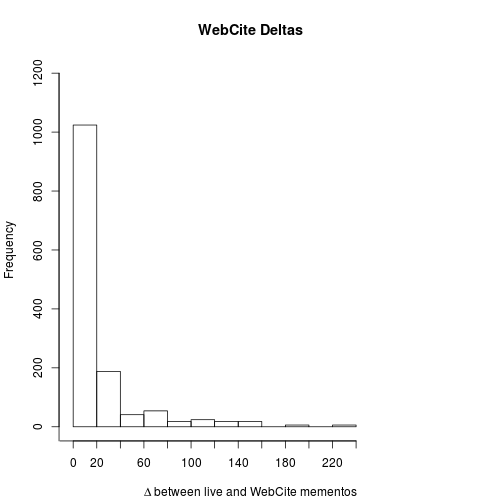
\includegraphics[width=270px]{./imgs/wcHisto.png}
\caption{Histogram of the memento vs live resource deltas in WebCite.}
\label{wchisto}
\end{figure}


\section{Conclusions}
\label{conclusion}
In this paper, we demonstrated that Web users (as represented by Mechanical Turk Workers) can correctly identify original mementos ($m_0$ vs $m_1$) 81\% of the time when presented with an original and manually damaged pair of mementos. After randomly selecting 100 URI-Ms from the Internet Archive TimeMaps of 1,861 URI-Rs, we show that turkers' assessment of damage does not match that of $M_m$; in fact, their perception of damage more closely aligns with a random selection than with $M_m$. 

To provide a damage metric closer to the perception of Web users, we proposed $D_m$, a damage calculation algorithm that estimates embedded resource importance to determine the perceived damage of mementos. Using turker evaluations, we showed that $D_m$ aligns with turker perception 32\% of the time when considering all {$\Delta D_m$} values -- an improvement of 17\% over $M_m$. If we limit {$\Delta D_m \textgreater$} 0.30, we achieve an agreement of 71\%, an improvement of 51\% over $M_m$. We show that the performance of $D_m$ is closer to that of the $m_0$ vs $m_1$ test than both $M_m$ and a random selection.

We used $D_m$ to measure the performance of the Internet Archive by measuring $\overline{D_m}$ of 1,861 URI-Rs. The average damage of the Internet Archive collection is 0.13 per memento and is missing 15\% of its embedded resources. Mementos are missing 2.05 important resources on average. The Internet Archive has gotten better at mitigating damage over time, reducing $D_m$ from 0.16 (1998) to 0.13 (2013). 

Page-at-a-time archivers perform differently than the Internet Archive. We measured mementos of our collection in WebCite, finding that the average damage of the collection is 0.397 per memento and is missing 18\% of its embedded resources. Mementos are missing 10.1 resources on average. Even though damage in the Internet Archive is improving, the damage in WebCite is getting worse, increasing $D_m$ from 0.375 (2007) to 0.475 (2013). 

We also demonstrate that JavaScript-dependent representations have a detrimental impact on $D_m$ and $M_m$. By using a crawl strategy in which JavaScript is executed during the crawl, damage in the resulting mementos can be improved by 13.5\%.

With $D_m$, archival services can evaluate their performance and the quality of their mementos. The archives could measure a selection of mementos (either randomly sampled or by identifying those missing a proportion of embedded resources, such as {$\Delta D_m \textgreater$} 0.30) for damage to determine whether or not they have been satisfactorily archived. That is, with this algorithm, the archives can provide the greatest damage improvement through targeted repair efforts (e.g., which mementos require additional attention to ensure proper archiving?). Archives can also use historical damage ratings of a URI-R to identify memento improvements or changes.

We also measured the damage of mementos in WebCite, and demonstrated that the damage in the Internet Archive ($\overline{D_m}$=0.128) is less than that in WebCite ($\overline{D_m}$=0.397). We know from previous works that WebCite does not archive JavaScript-dependent representations easily. We also measured Archive.today to determine the fidelity of an archival service that makes an effort to capture JavaScript dependent representations. We found that Archive.today had a delta of 19.9 embedded resources between mementos and live resources, while WebCite had a delta of 21.6. This shows that Archive.today provides a higher fidelity memento than WebCite.

This is a preliminary investigation of memento damage. We have shown that percentage of embedded resources missing is not an accurate representation of damage and have proposed a more accurate metric.  Our future work will continue to improve upon the metric by using larger datasets, more turkers, and machine learning to further hone $D_m$. This will include a refinement of the relative weights of the embedded resources (e.g., the relative importance of CSS vs. images). We will also investigate the cumulative damage rating over time. For example, a logo that never changes over a 5 year period could have increased importance due to its use over multiple mementos. We plan to also measure the damage improvement of mementos if embedded resources are retroactively captured and included in past mementos. This cumulative damage improvement can help identify embedded resources that should be targeted by archives.



\section{Acknowledgments}
This work supported in part by the National Science Foundation (NSF) (IIS 1009392), the Library of Congress, and the National Endowment for the Humanities (NEH) Digital Humanities Implementation Grant (DHIG) (HK-50181-14).


%\bibliographystyle{abbrv}
\bibliographystyle{spmpsci}
\bibliography{_mybibtex} 
%\bibliography{_mybibtex}  





\end{document}
% end of file template.tex

